%% ------------------------------------------------------------------------- %%
\chapter{Processamento}
\label{cap:processamento}

Esse capítulo apresenta como as teorias do capítulo anterior foram utilizadas para obtenção 
dos resultados que serão discutidos no próximo capítulo.

%% ------------------------------------------------------------------------- %%
\section{Conjunto de Dados}
\index{Conjunto de Dados}
\label{sec:dados}

Os dados utilizados foram os dados do catálogo \gls{iscgem} \citep{storchak_2013} 
para a América do Sul e 
os dados do \glsdesc{bsb2013} \citep{bsb2013} para o Brasil.

O dados são texto e formatados em arquivos de \gls{csv}.

A figura \ref{fig:eq_record} ilustra o número de registros de tremores por ano nos dois catálogos.

\begin{figure}[H]
	\centering
	\begin{subfigure}[b]{0.48\textwidth}
		  	\centering
			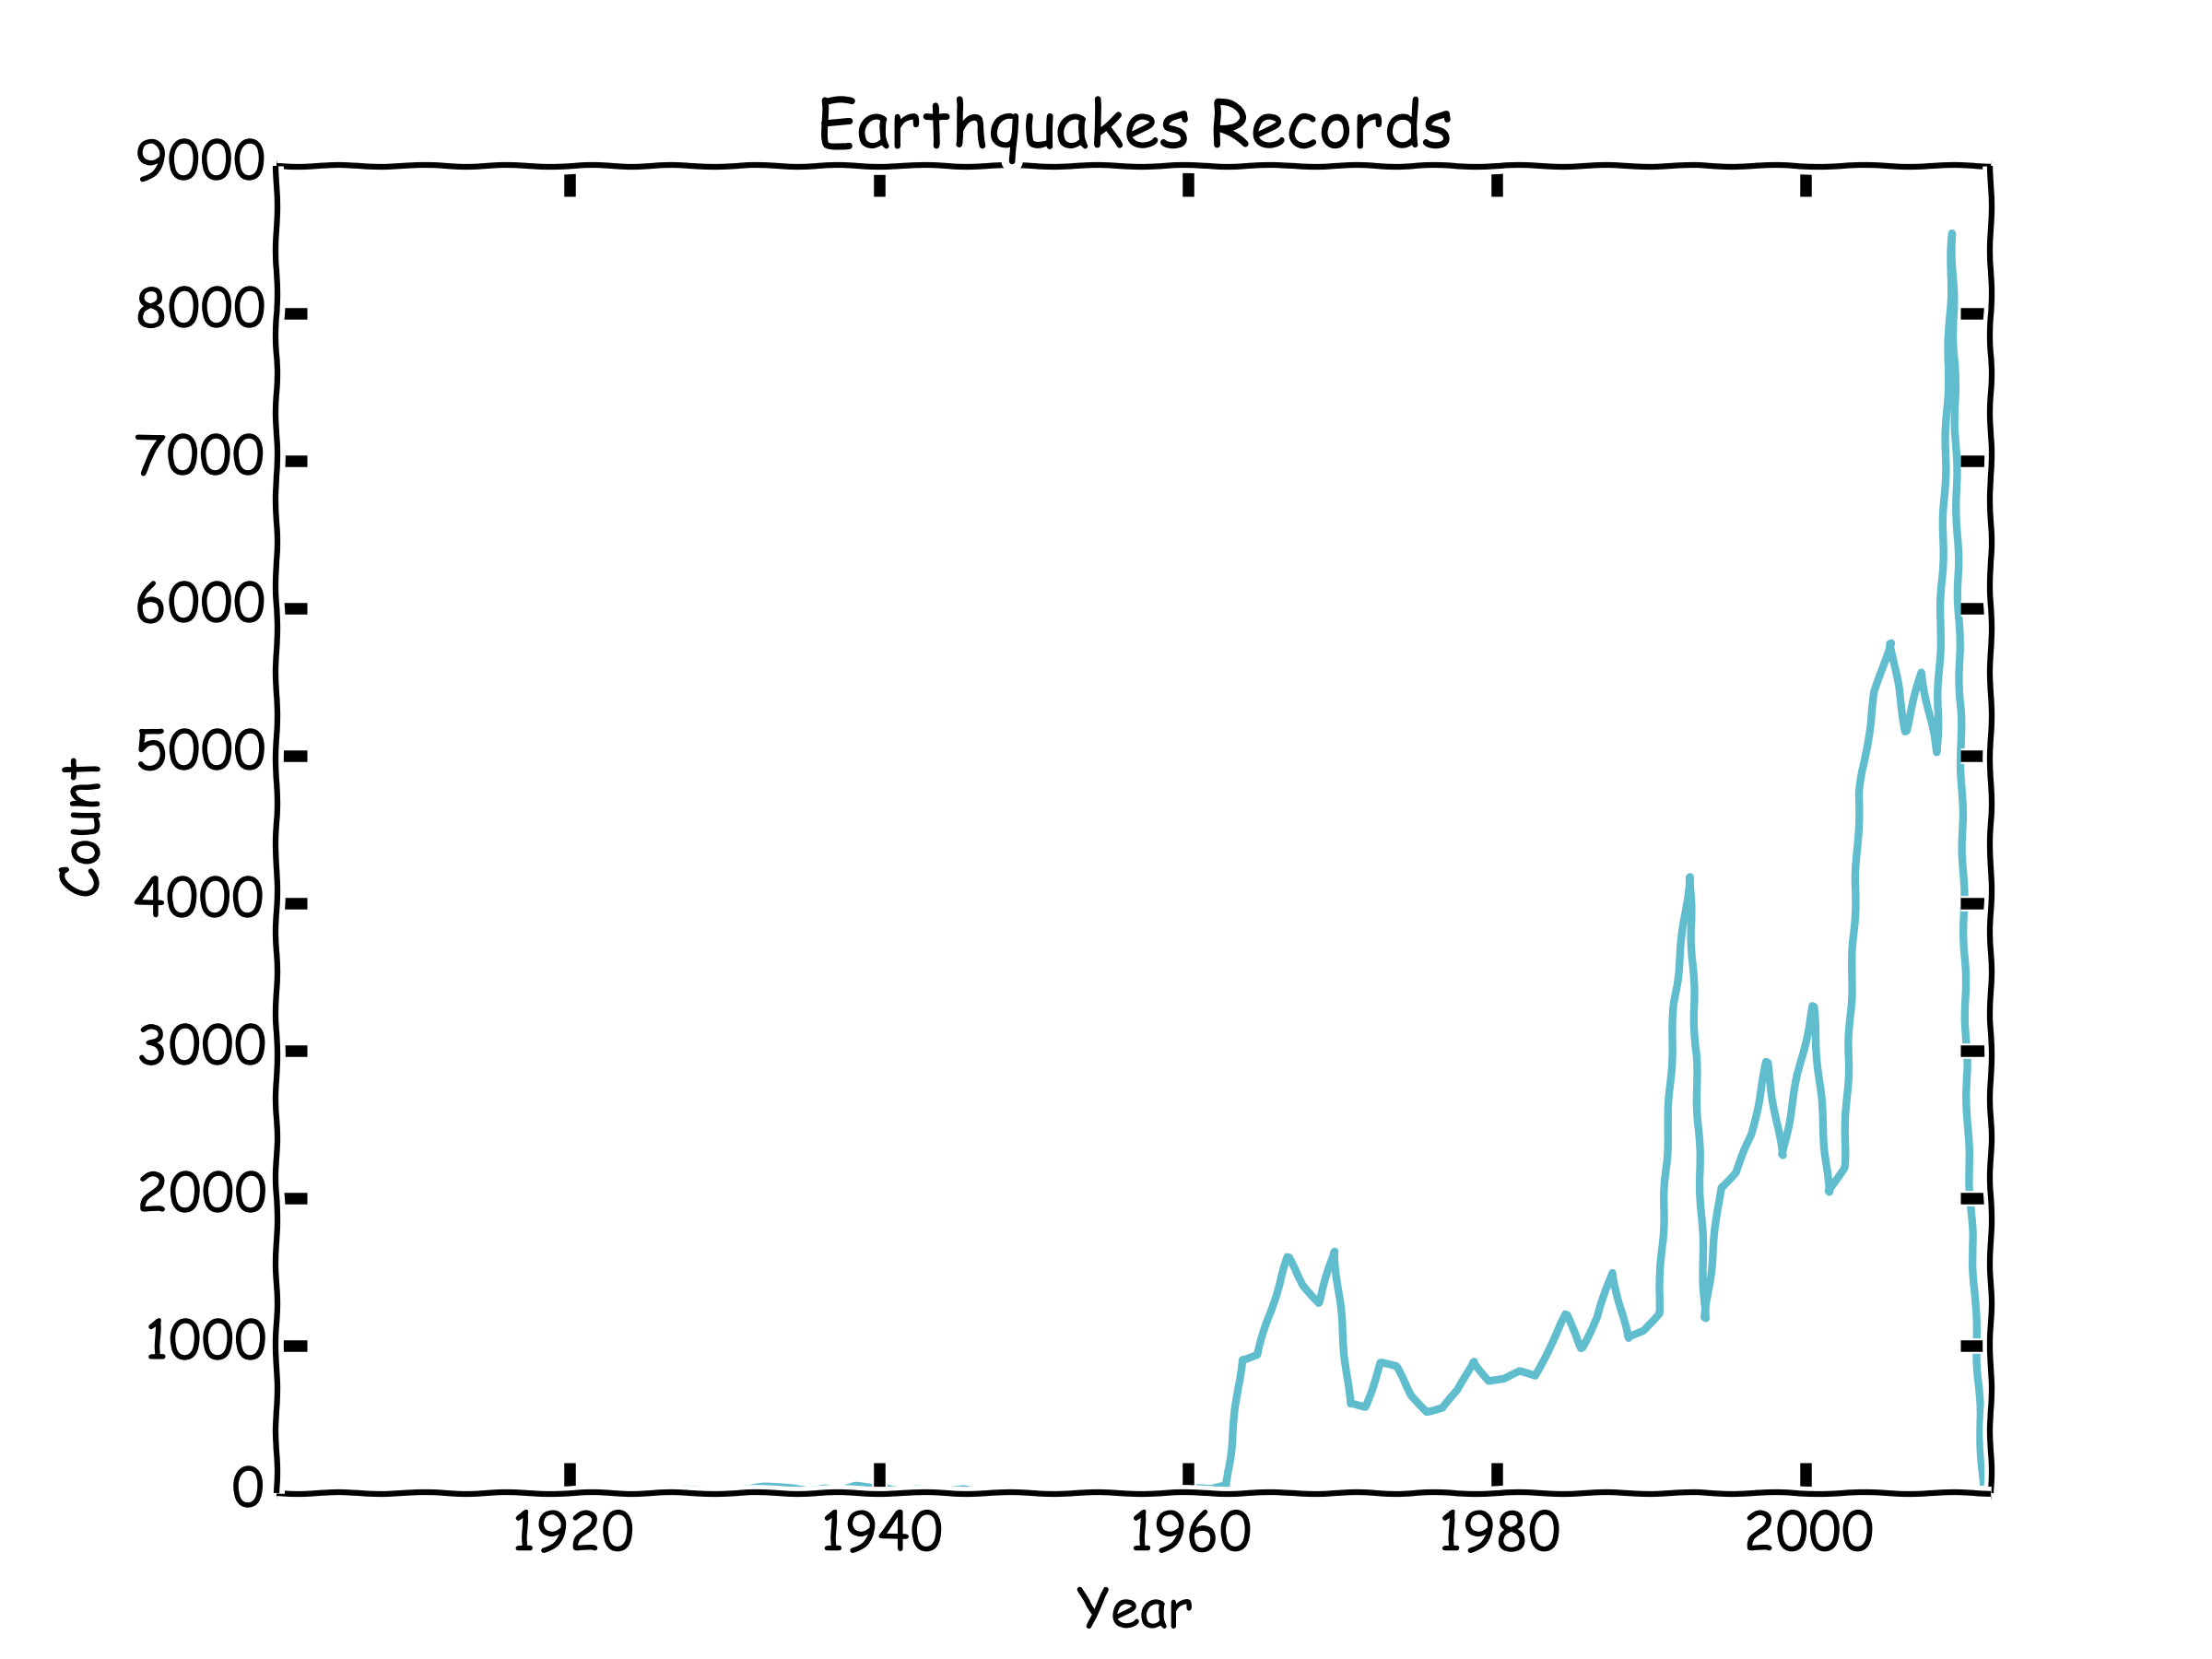
\includegraphics[width=1.00\textwidth]{hmtk_sa3_rate}
			\subcaption{Número de tremores registrados por ano, \gls{iscgem}}
			\label{fig:sa_eq_record}
	\end{subfigure}%
	\quad %~ %add desired spacing between images, e. g. ~, \quad, \qquad, \hfill etc.
	\begin{subfigure}[b]{0.48\textwidth}
		  	\centering
			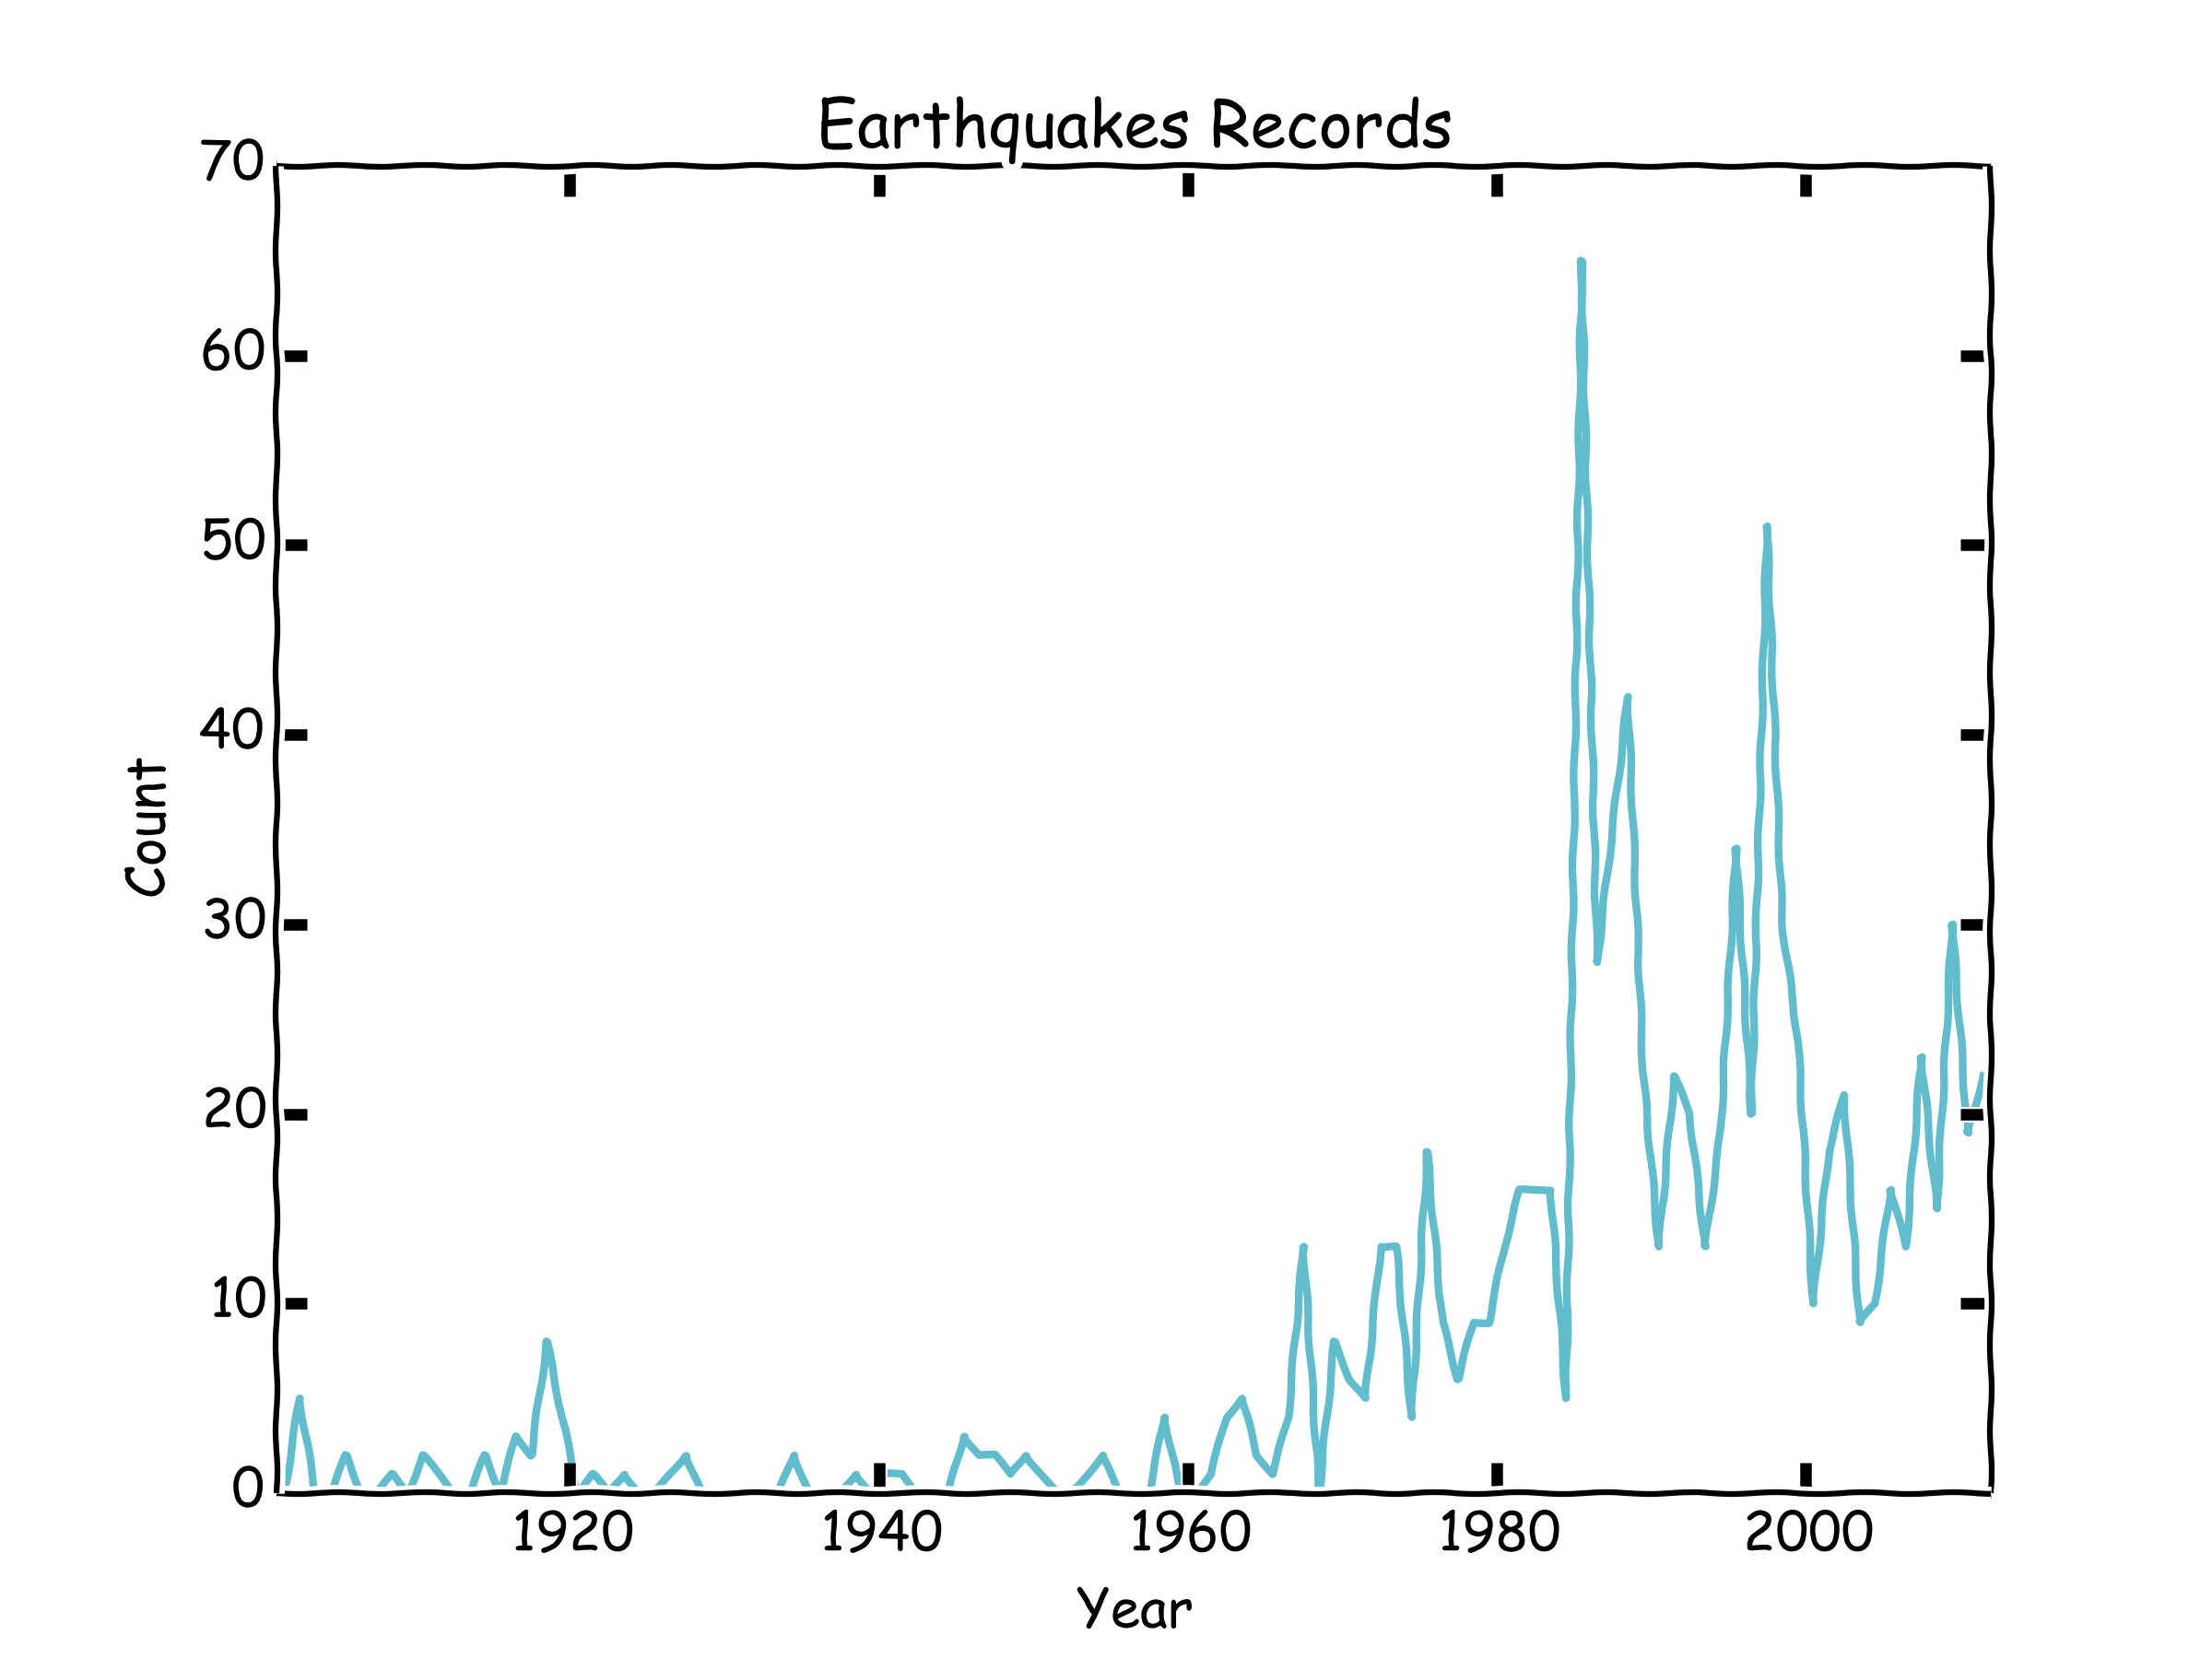
\includegraphics[width=1.00\textwidth]{hmtk_bsb2013_rate}
			\subcaption{Número de tremores registrados por ano, \gls{bsb2013}}
			\label{fig:br_eq_record}
    \end{subfigure}%
	\caption{Número de tremores registrados por ano após 1900}
	\label{fig:eq_record}
\end{figure}

Em ambos é possível notar um incremento do número de registros de sismos com o passar dos anos, 
além de algumas variações bem destacadas em períodos reduzidos de poucos anos.



%% ------------------------------------------------------------------------- %%
\subsection{Catálogo ISC-GEM}
\index{Conjunto de Dados!ISC-GEM}
\label{sec:data_source}

O \glsdesc{iscgem} versão 1.04 possui licença CC-BY-SA e é fruto da redeterminação de parâmetros
dos terremotos com os dados disponíveis no ISC-GEM e de um detalhado estudo para que ao menos um valor de
magnitude $\gls{sym:Mw}$ estivesse disponível com incertezas.

Possui um pouco mais de 110 000 registros.  

\subsection{Boletim Sísmico Brasileiro}
\index{Conjunto de Dados!BSB}
\label{sec:data_source2}

O \glsdesc{bsb} \citep{bsb2013}, versão 2013.08 possui licença CC-BY e é fruto do esforço de compilação de
dados e determinação de epicentros e magnitudes que contou com a colaboração de várias instituições
como o \gls{obsis} da \gls{unb}, o \gls{ipt}, a \gls{unesp}, a \gls{ufrn} liderados pelo \gls{iag} da \gls{usp}.

Possui algo em torno de 900 registros.

%% ------------------------------------------------------------------------- %%

\section{Ferramentas}
\index{Ferramentas}
\label{sec:ferramentas}

As ferramentas utilizadas para as análises e cálculos apresentados nesse texto
foram de código aberto.
Utilizou-se o Latex para a edição do texto, o software de processamento de dados
geoespacial QGIS, o console do Linux BASH, a IDE Eclipse, o git/GitHub para o controle de versao,

O iPython como console interativo, a MatplotLib e Basemap para o gráficos, 
a SciPy para um conjunto de funções científicas e estatísticas, a shapely e gdal
para lidar com objetos com atributos geométricos.


%% ------------------------------------------------------------------------- %%
\subsection{Linguagens de Programação}
\index{Linguagens de Programação}
\label{sec:linguagens}

A principal linguagem de programação utilizada foi Python.

Os códigos-fonte dos modelos de Woo e de Helmstetter foram providos pelos autores
e estão em Fortran. O método de Frankel estava disponível em Python.


%% ------------------------------------------------------------------------- %%
\subsection{Programas de Computador}
\index{Ferramentas!programas}\index{software}
\label{sec:software}

O programa mais comum para esse tipo de análise costuma ser o CRISIS \citep{crisis_2007} nas suas mais diversas
versões. Como nesse trabalho a opção foi por código aberto, poderia ter se optado pelo 
\gls{opensha}\footnote{\url{http://www.opensha.org}} que é escrito em Java.

A intenção no entanto foi provar o conjunto de tecnologias mantido pela fundação \gls{gem}
que para o cálculo de ameaça e rísco sísmico que é o \gls{oq} \citep{pagani_2014}.

O código do \gls{oq} está abertamente disponível para consulta e clonagem no GitHub
\footnote{\url{https://github.com/GEM}}.

O ecossistema do \gls{oq} é ilustrado na figura a seguir:

\begin{figure}[!h]
  \centering
  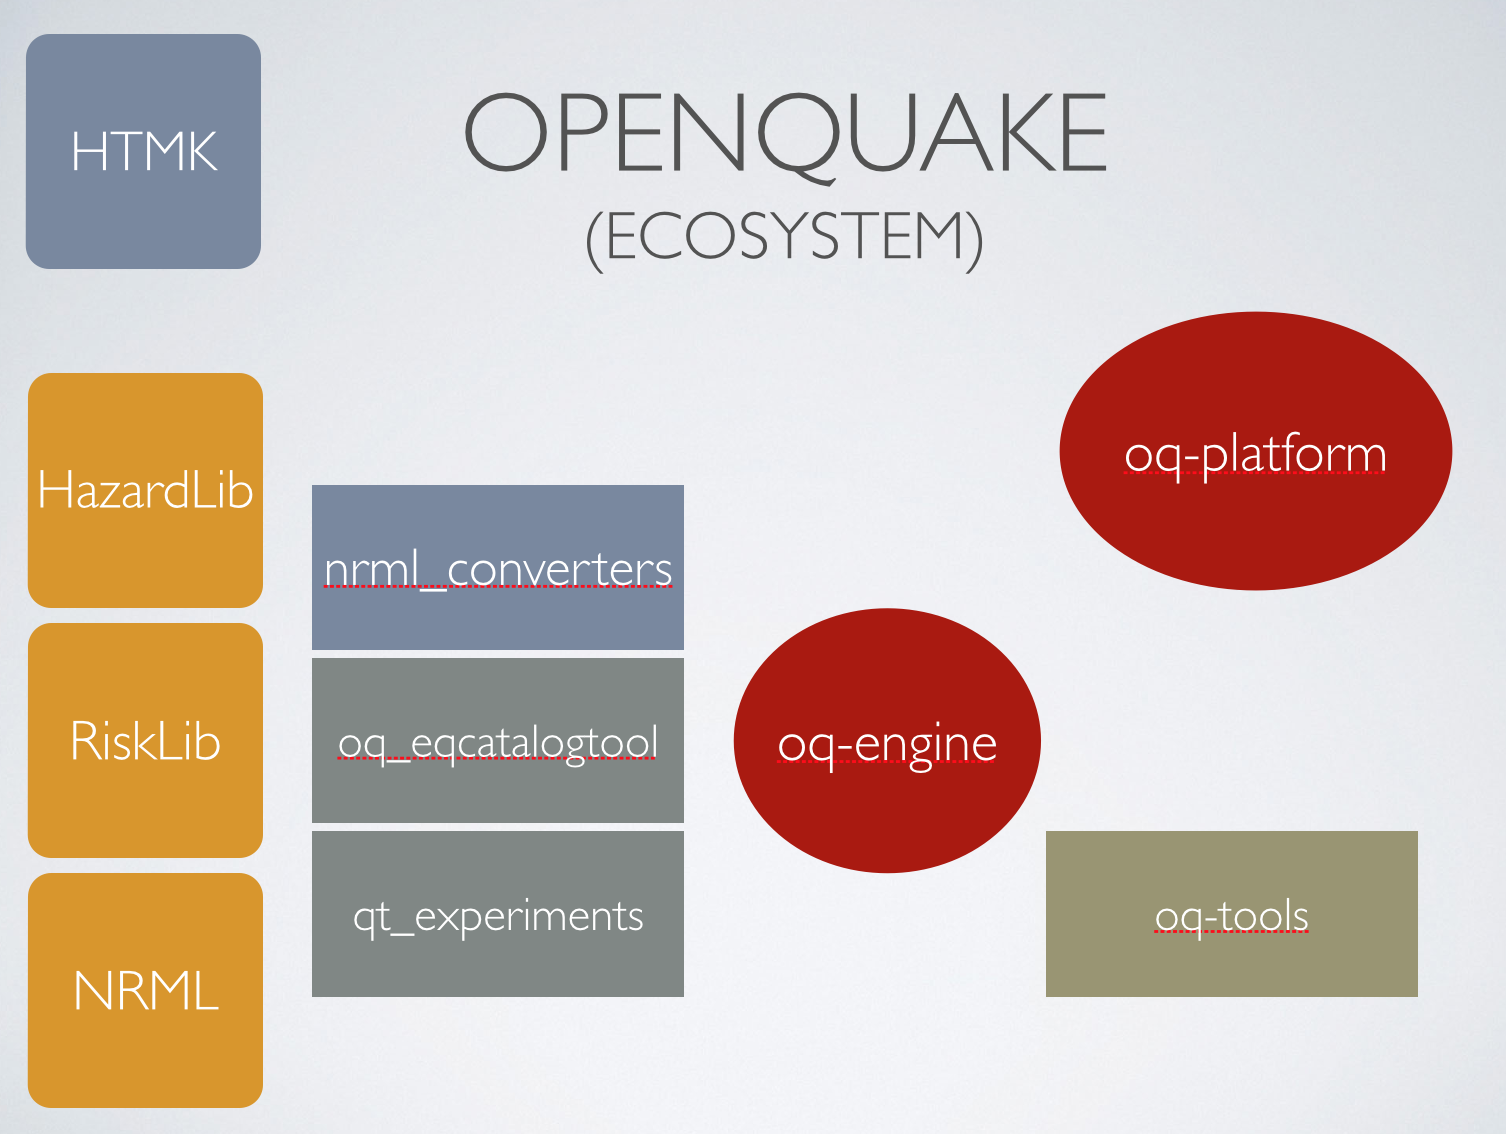
\includegraphics[width=.80\textwidth]{oq_ecosystem} 
  \caption{Ecossistema de módulos, bibliotecas e utilitários do OpenQuake}
  \label{fig:oq} 
\end{figure}

O destaque em vermelho na figura \ref{fig:oq} fica para o \gls{oqe} que executa as simulações de cada tronco da
arvore-lógica e as usa para calcular o cenário de risco e armazenar o resultado.
Faz isso distribuindo o processamento em tarefas e permitindo escalar o cálculo.

A \gls{oqp} permite interagir com os dados armazenados e gerenciados na nuvem, como catálogos, 
falhas, dados de esforços, fontes sismogênicas e suas geometrias usados em cálculos de ameaça/risco.
Permite também interagir com o resultado do cálculo, visualizando mapas de ameaça e curvas de intensidade.

%% ------------------------------------------------------------------------- %%
\subsection{Bibliotecas de Funções}
\index{ferramentas!bibliotecas}
\label{sec:bibliotecas}

Em amarelo na figura \ref{fig:oq} está biblioteca a \gls{hl} que contém toda lógica e ciência para o cálculo de ameaça,
como os tipos de fontes sísmogênicas, as \gls{mfd}, as \glspl{gmpe}, etc. 

Está também a \gls{rl}
que contém os modelos de vulnerabilidade e exposição para a análise de risco. 

E por último,
a \gls{nrml} que é a sintaxe da linguagem de representação das árvores-lógicas, fontes sísmicas e
resultados, como mapas de risco, espectro de alguma medida de intensidade, etc. 


%% ------------------------------------------------------------------------- %%
\subsection{Implementações e Novos Códigos}
\index{Implementações e novos códigos }
\label{sec:implementacao}

Incluído no suporte da fundação \gls{gem} está a manutenção de um Comitê Científico
que desenvolve ferramentas auxiliares adicionais como conversores, ferramentas para trabalho com 
o catálogo, ferramentas gráficas, entre outras para interação com o
\gls{oq} como pode ser visto na figura \ref{fig:oq} em azul, cinza e bege.

Uma dessas ferramentas em especial é o \gls{hmtk} \citep{weatherill_2012, weatherill_2014-1} que facilita todo o
processo de modelagem da \gls{psha} como a remoção de agrupamentos, a caracterização de zonas sísmicas,  
a visualização da evolução da taxa de sismicidade, a análise da magnitude de completude e
estimativa do \emph{valor-b}.

O \gls{hmtk} já trazia um módulo para trabalhar com a sismicidade que usava as \gls{smoothing}
implementando o método de \citet{frankel_1995}. E é na \gls{hmtk} que se pretende
contribuir com a implementação dos métodos de \citet{woo_1996} e de \citet{helmstetter_2012}.
 
%% ------------------------------------------------------------------------- %%
\section{Pré-Processamento}
\index{pré-processamento}
\label{sec:pre_processamento}

Para aplicar as \gls{smoothing} no conjunto de dados é necessário alguns primeiros procedimendos.

%% ------------------------------------------------------------------------- %%
\subsection{Controle de Qualidade}
\index{pre-processamento!controle de qualidade}
\label{sec:qualicontrol}

A primeira coisa ser fazer no conjunto de dados é uma checagem geral.

Nessa hora é preciso observar se não há pontos com coordenadas erradas, invertidas, faltando valores de dias ou horas.

É recomendado também fazer uma varredura em busca de vieses no catálogo \citep{van_stiphout_2010}.
Isso é feito com, por exemplo, um histogramas do dia da semana da ocorrência dos tremores em busca
de algum descréscimo em fins de semana que seriam um provável indicativo de contaminação do catálogo 
por atividade humana, por exemplo explosões em pedreiras. 
Também é possível fazer um histograma para observar a
distribuição do horário de ocorrência durante o dia, 
ou mesmo da profundidade para estimar a resolução do catálogo
nesse quesito. A figura \ref{fig:qc_histograms} apresenta alguns dos histogramas sugeridos para a análise
exploratória dos dados dos catálogos.

\begin{figure}[H]
	\centering
	\begin{subfigure}[b]{0.45\textwidth}
		  	\centering
			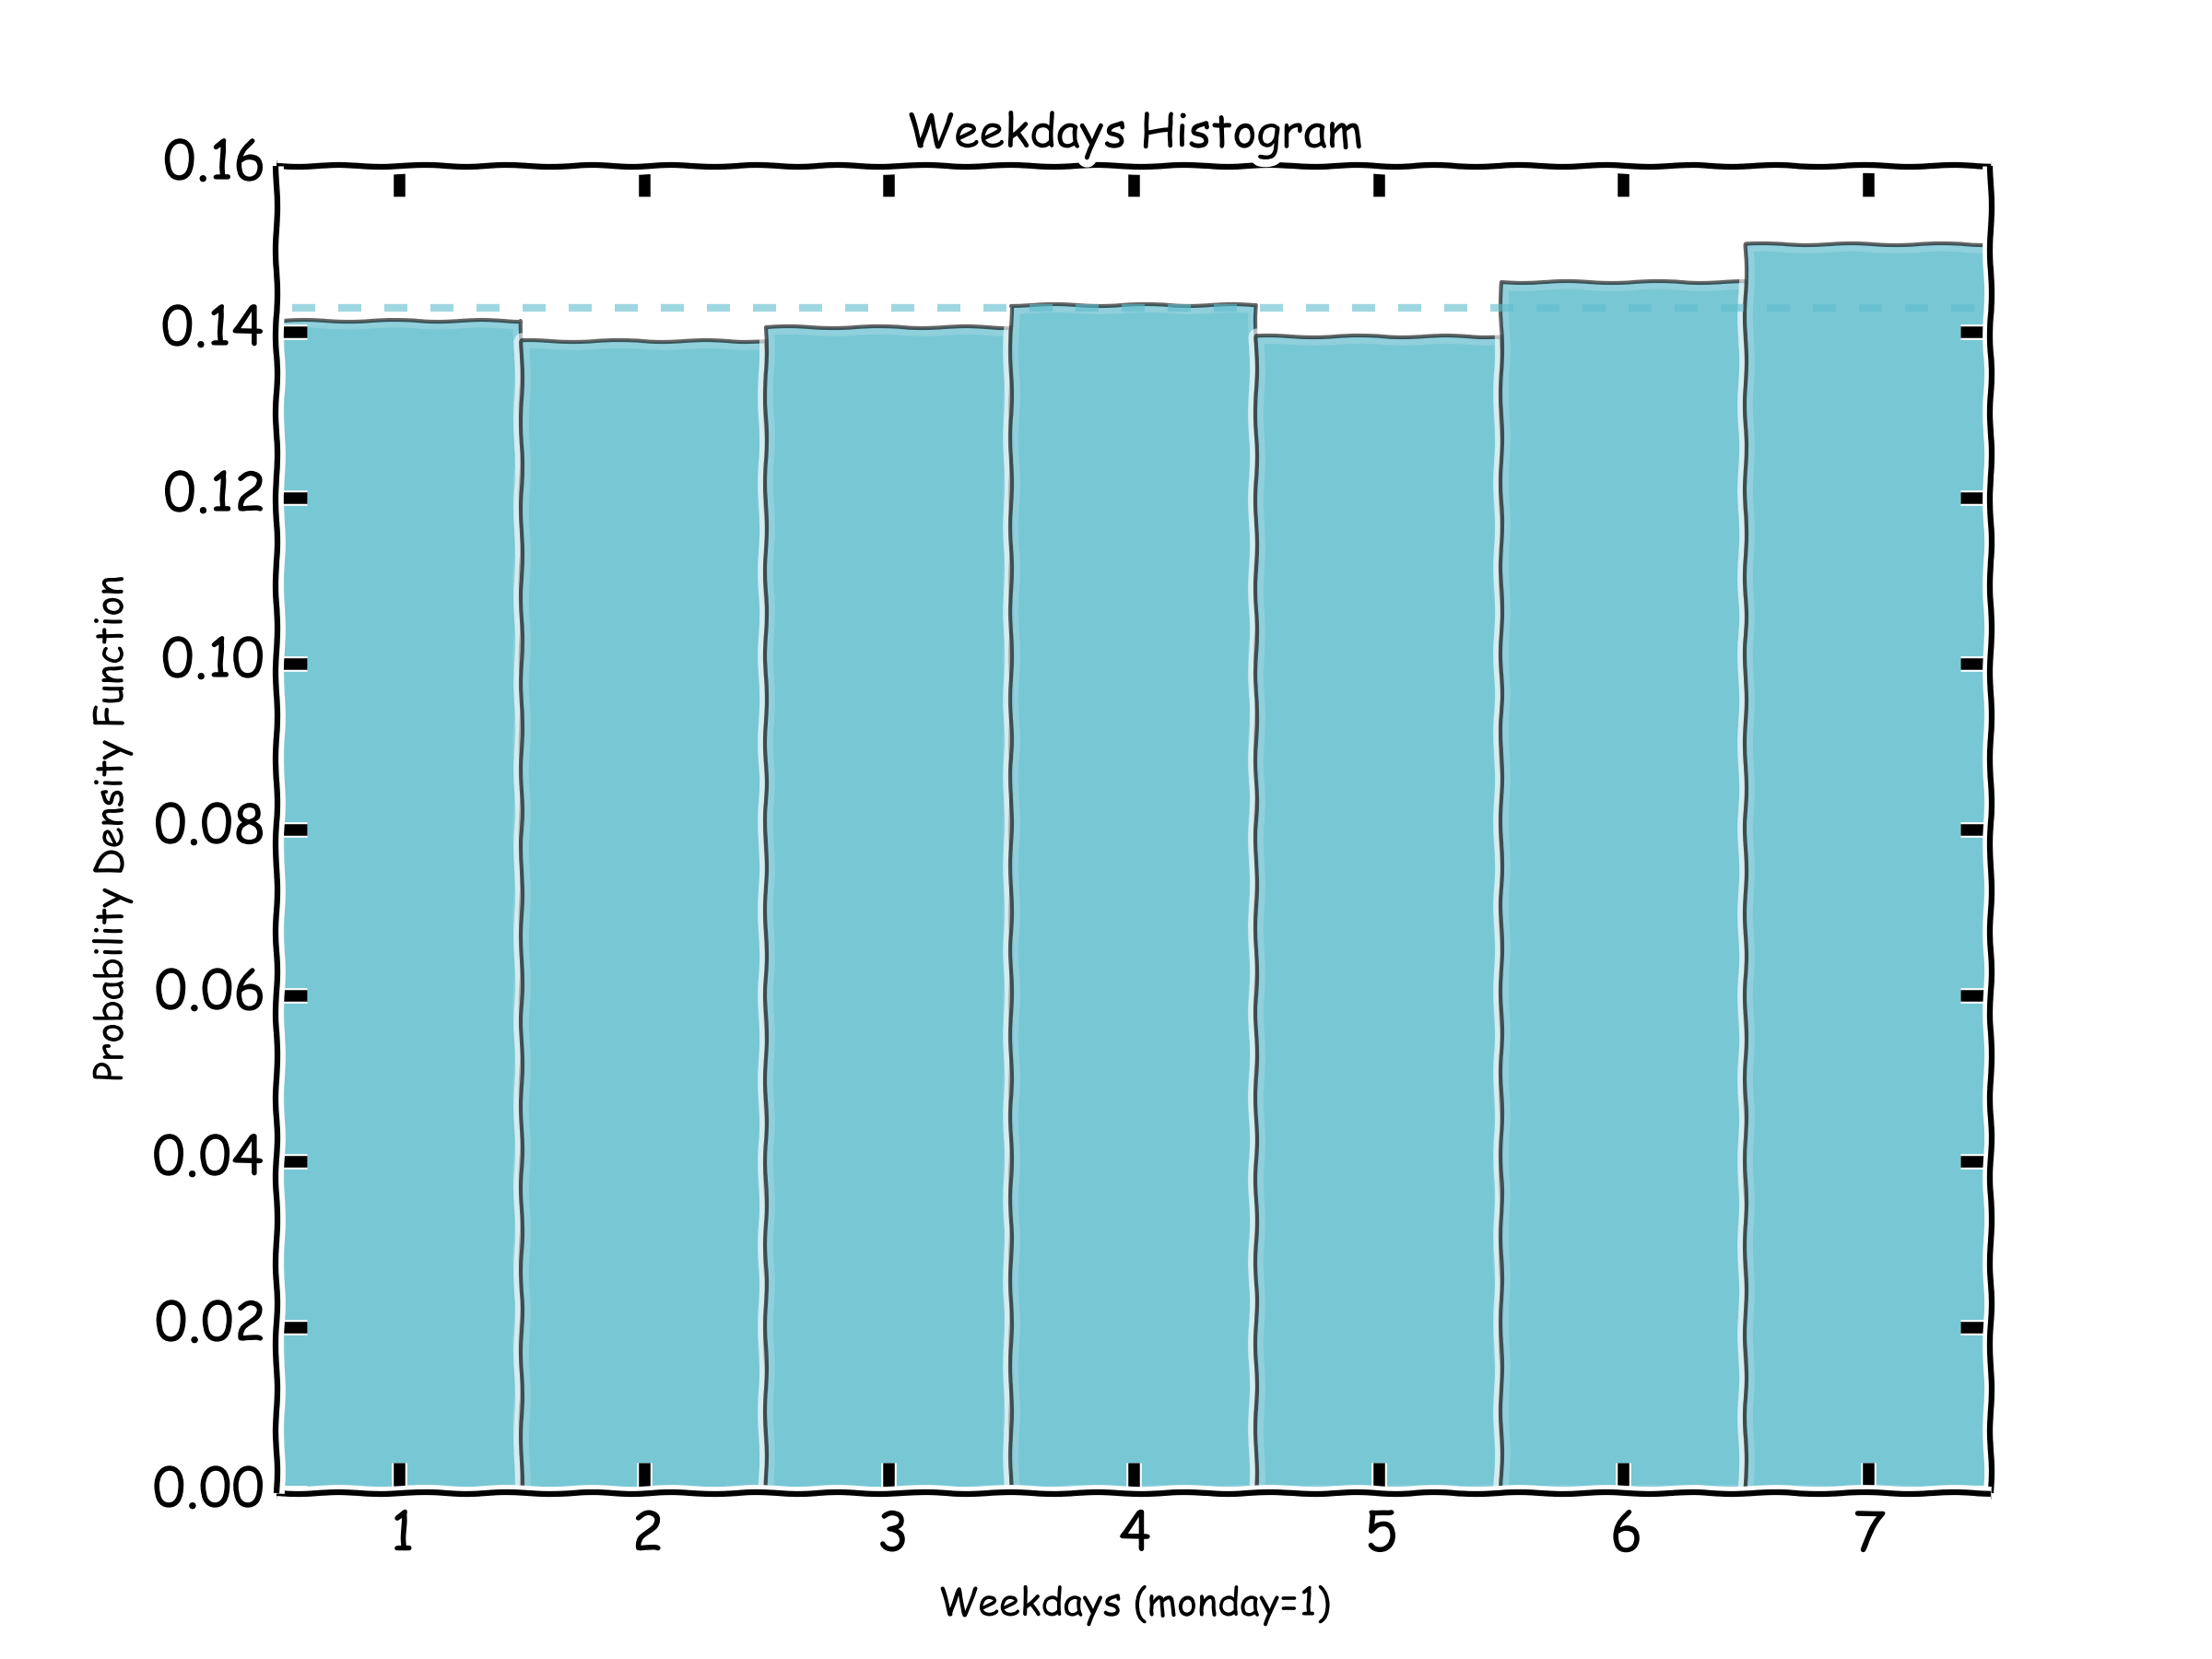
\includegraphics[width=1.00\textwidth]{hmtk_sa3_weekday}
			\subcaption{Distribuição dos tremores nos dias da semana, \gls{iscgem}}
			\label{fig:sa_week_hist}
	\end{subfigure}%
	\quad %~ %add desired spacing between images, e. g. ~, \quad, \qquad, \hfill etc.
	\begin{subfigure}[b]{0.45\textwidth}
		  	\centering
			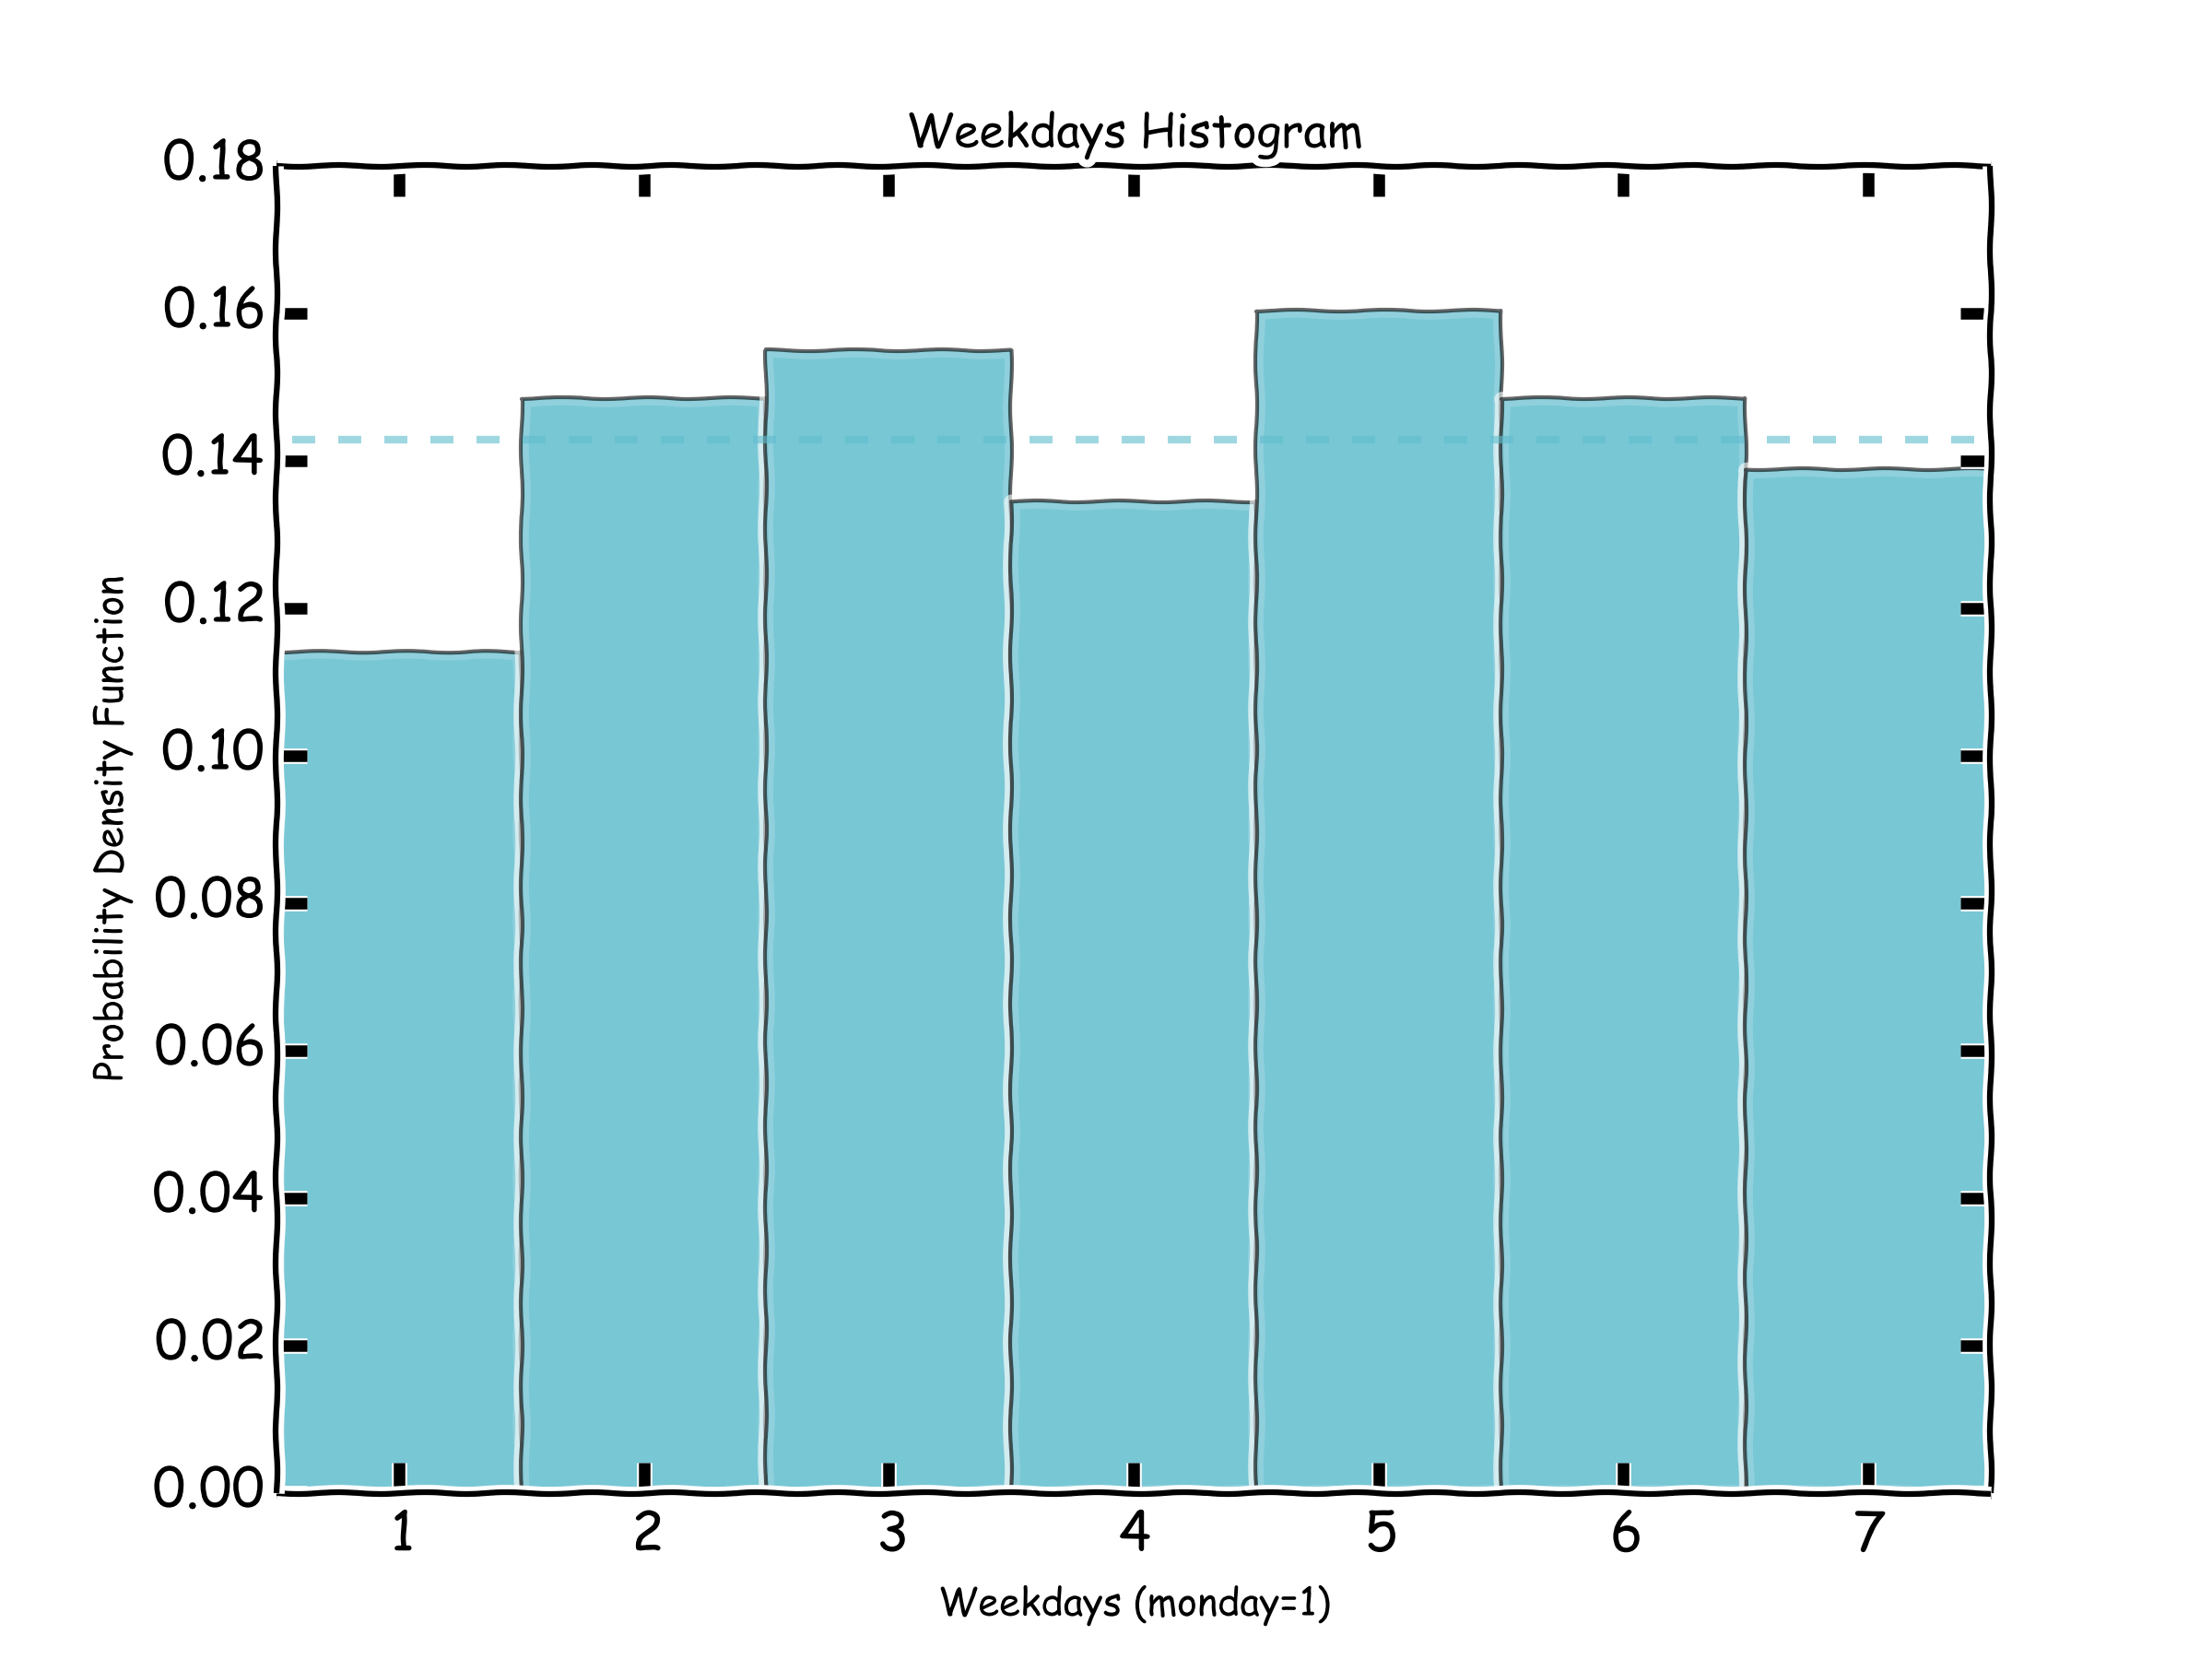
\includegraphics[width=1.00\textwidth]{hmtk_bsb2013_weekday}
			\subcaption{Distribuição dos tremores nos dias da semana, \gls{bsb2013}}
			\label{fig:br_week_hist}
    \end{subfigure}%
        %~ %add desired spacing between images, e. g. ~, \quad, \qquad, \hfill etc.
          %(or a blank line to force the subfigure onto a new line)
          
 	\begin{subfigure}[b]{0.45\textwidth}
		  	\centering
			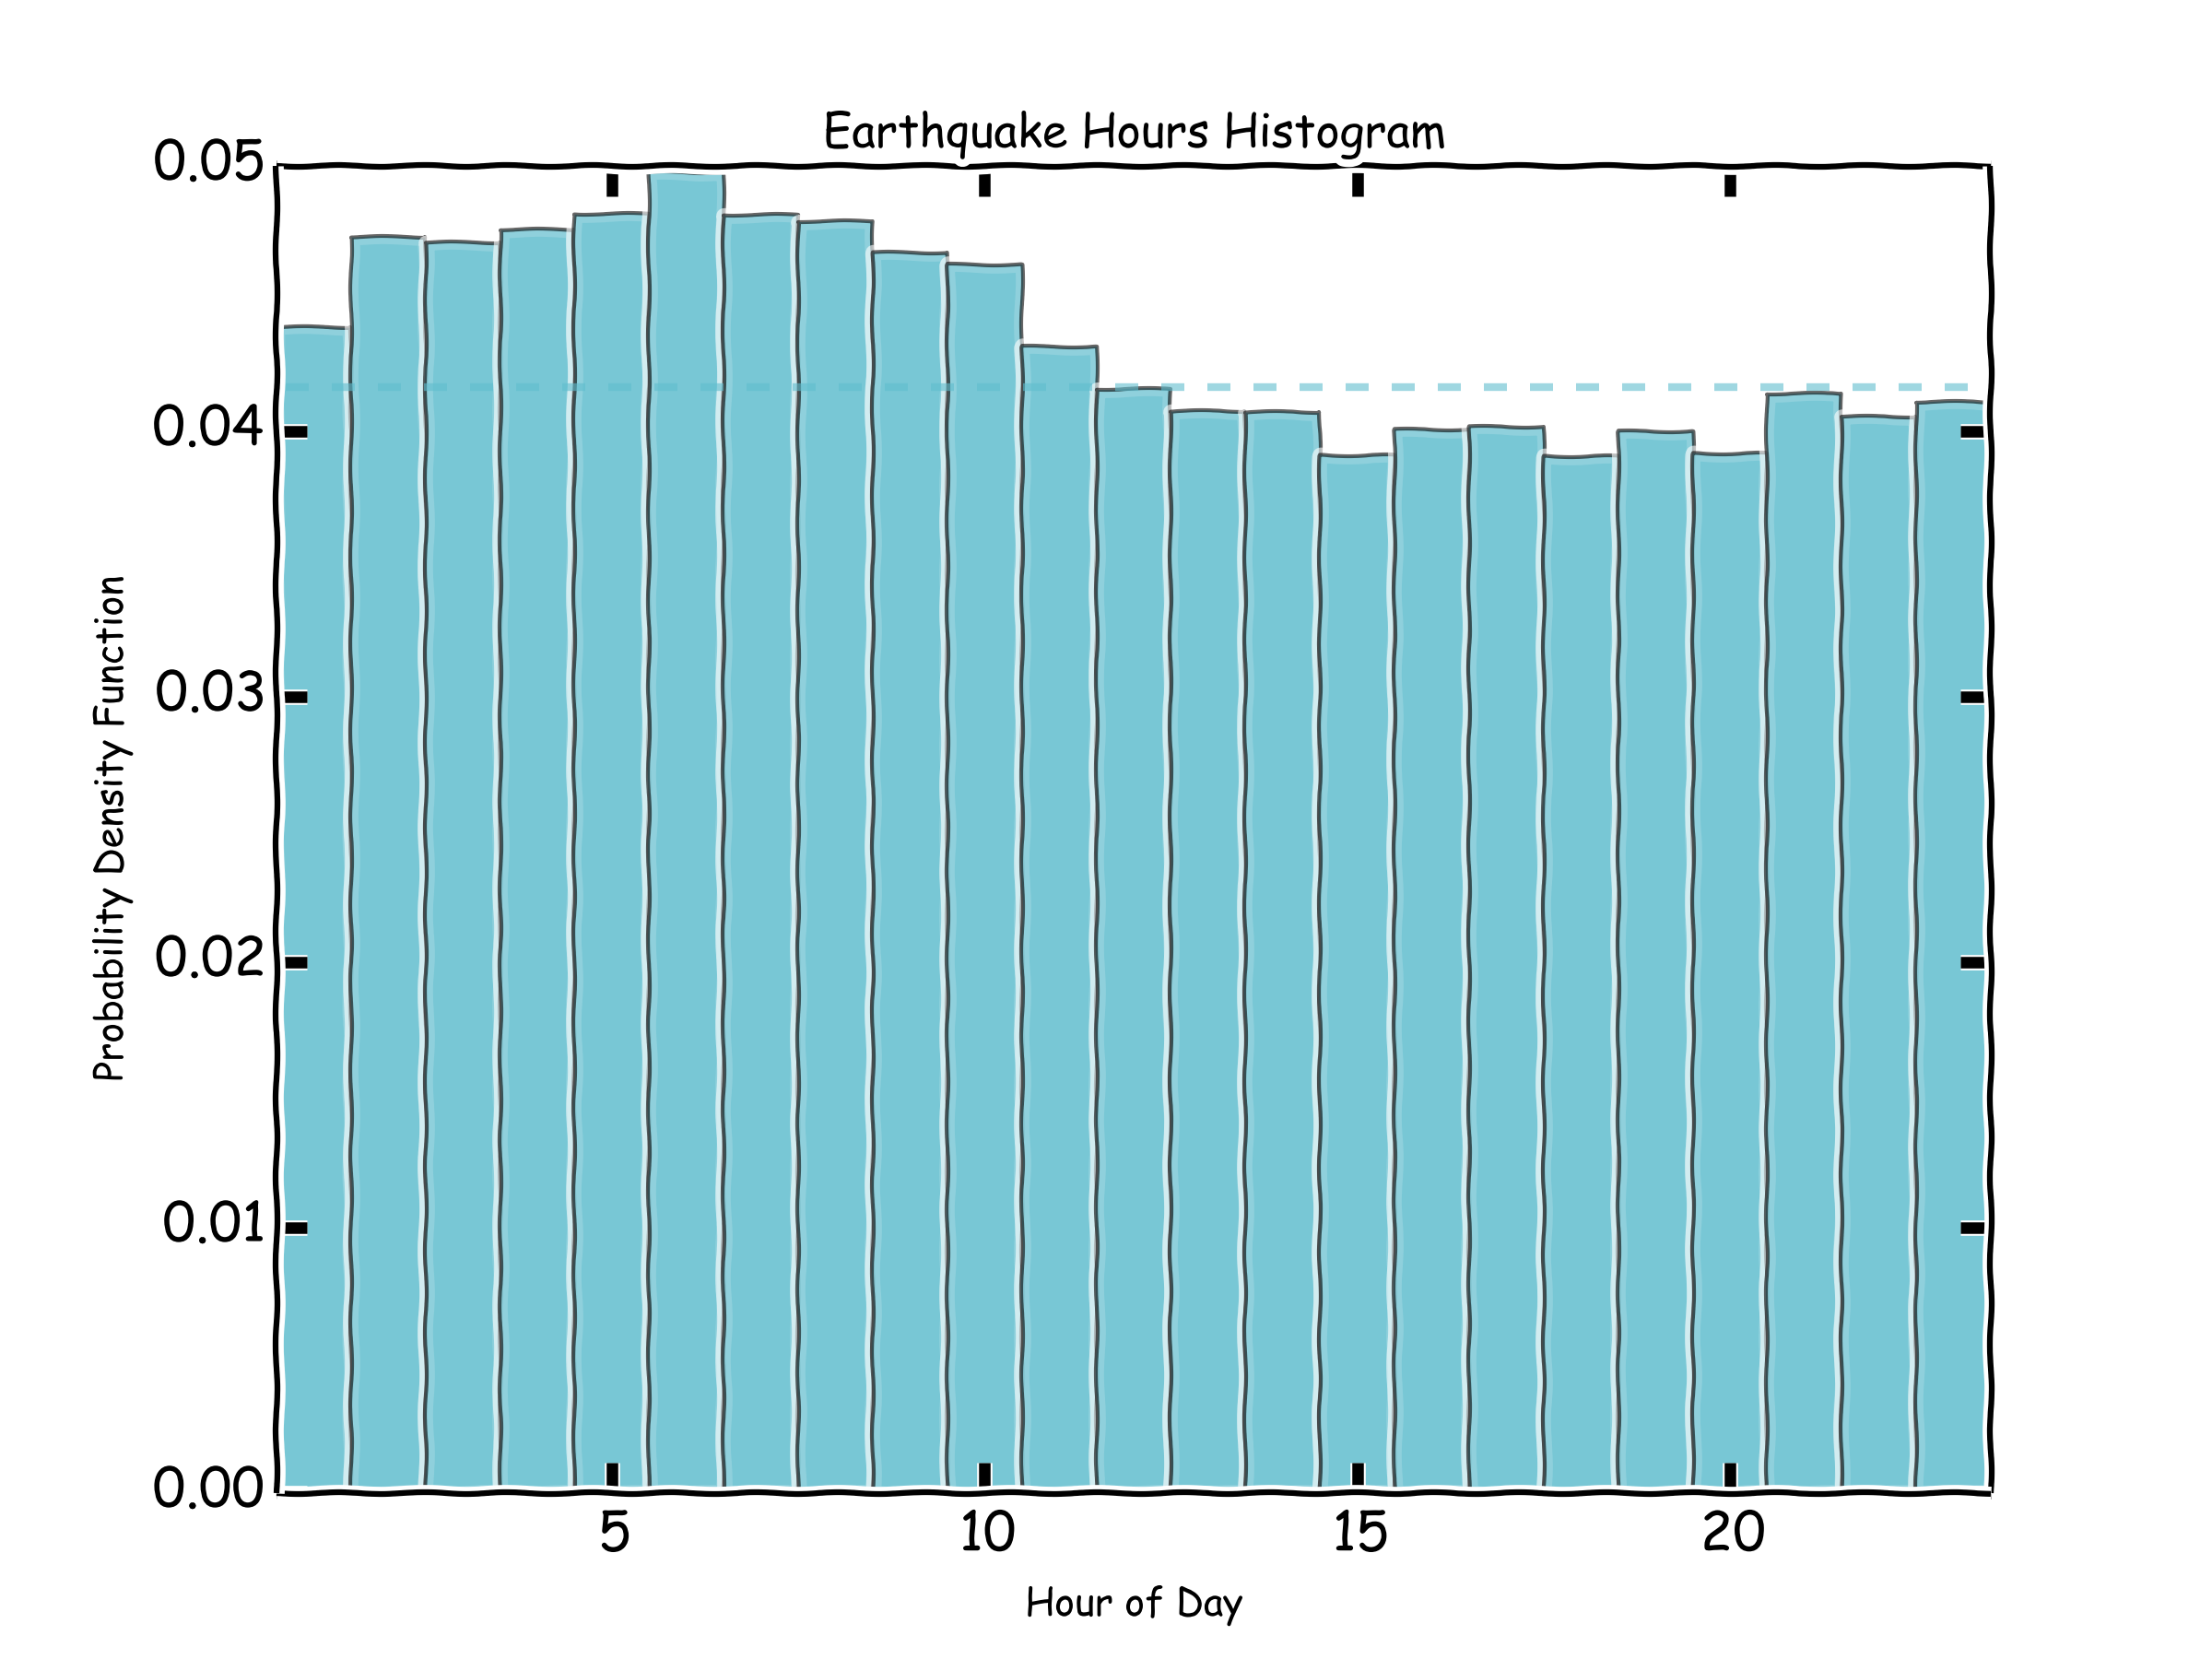
\includegraphics[width=1.00\textwidth]{hmtk_sa3_hour}
			\subcaption{Distribuição do horário de ocorrência dos tremores, \gls{iscgem}}
			\label{fig:sa_hour_hist}
	\end{subfigure}%
	\quad %~ %add desired spacing between images, e. g. ~, \quad, \qquad, \hfill etc.
	\begin{subfigure}[b]{0.45\textwidth}
		  	\centering
			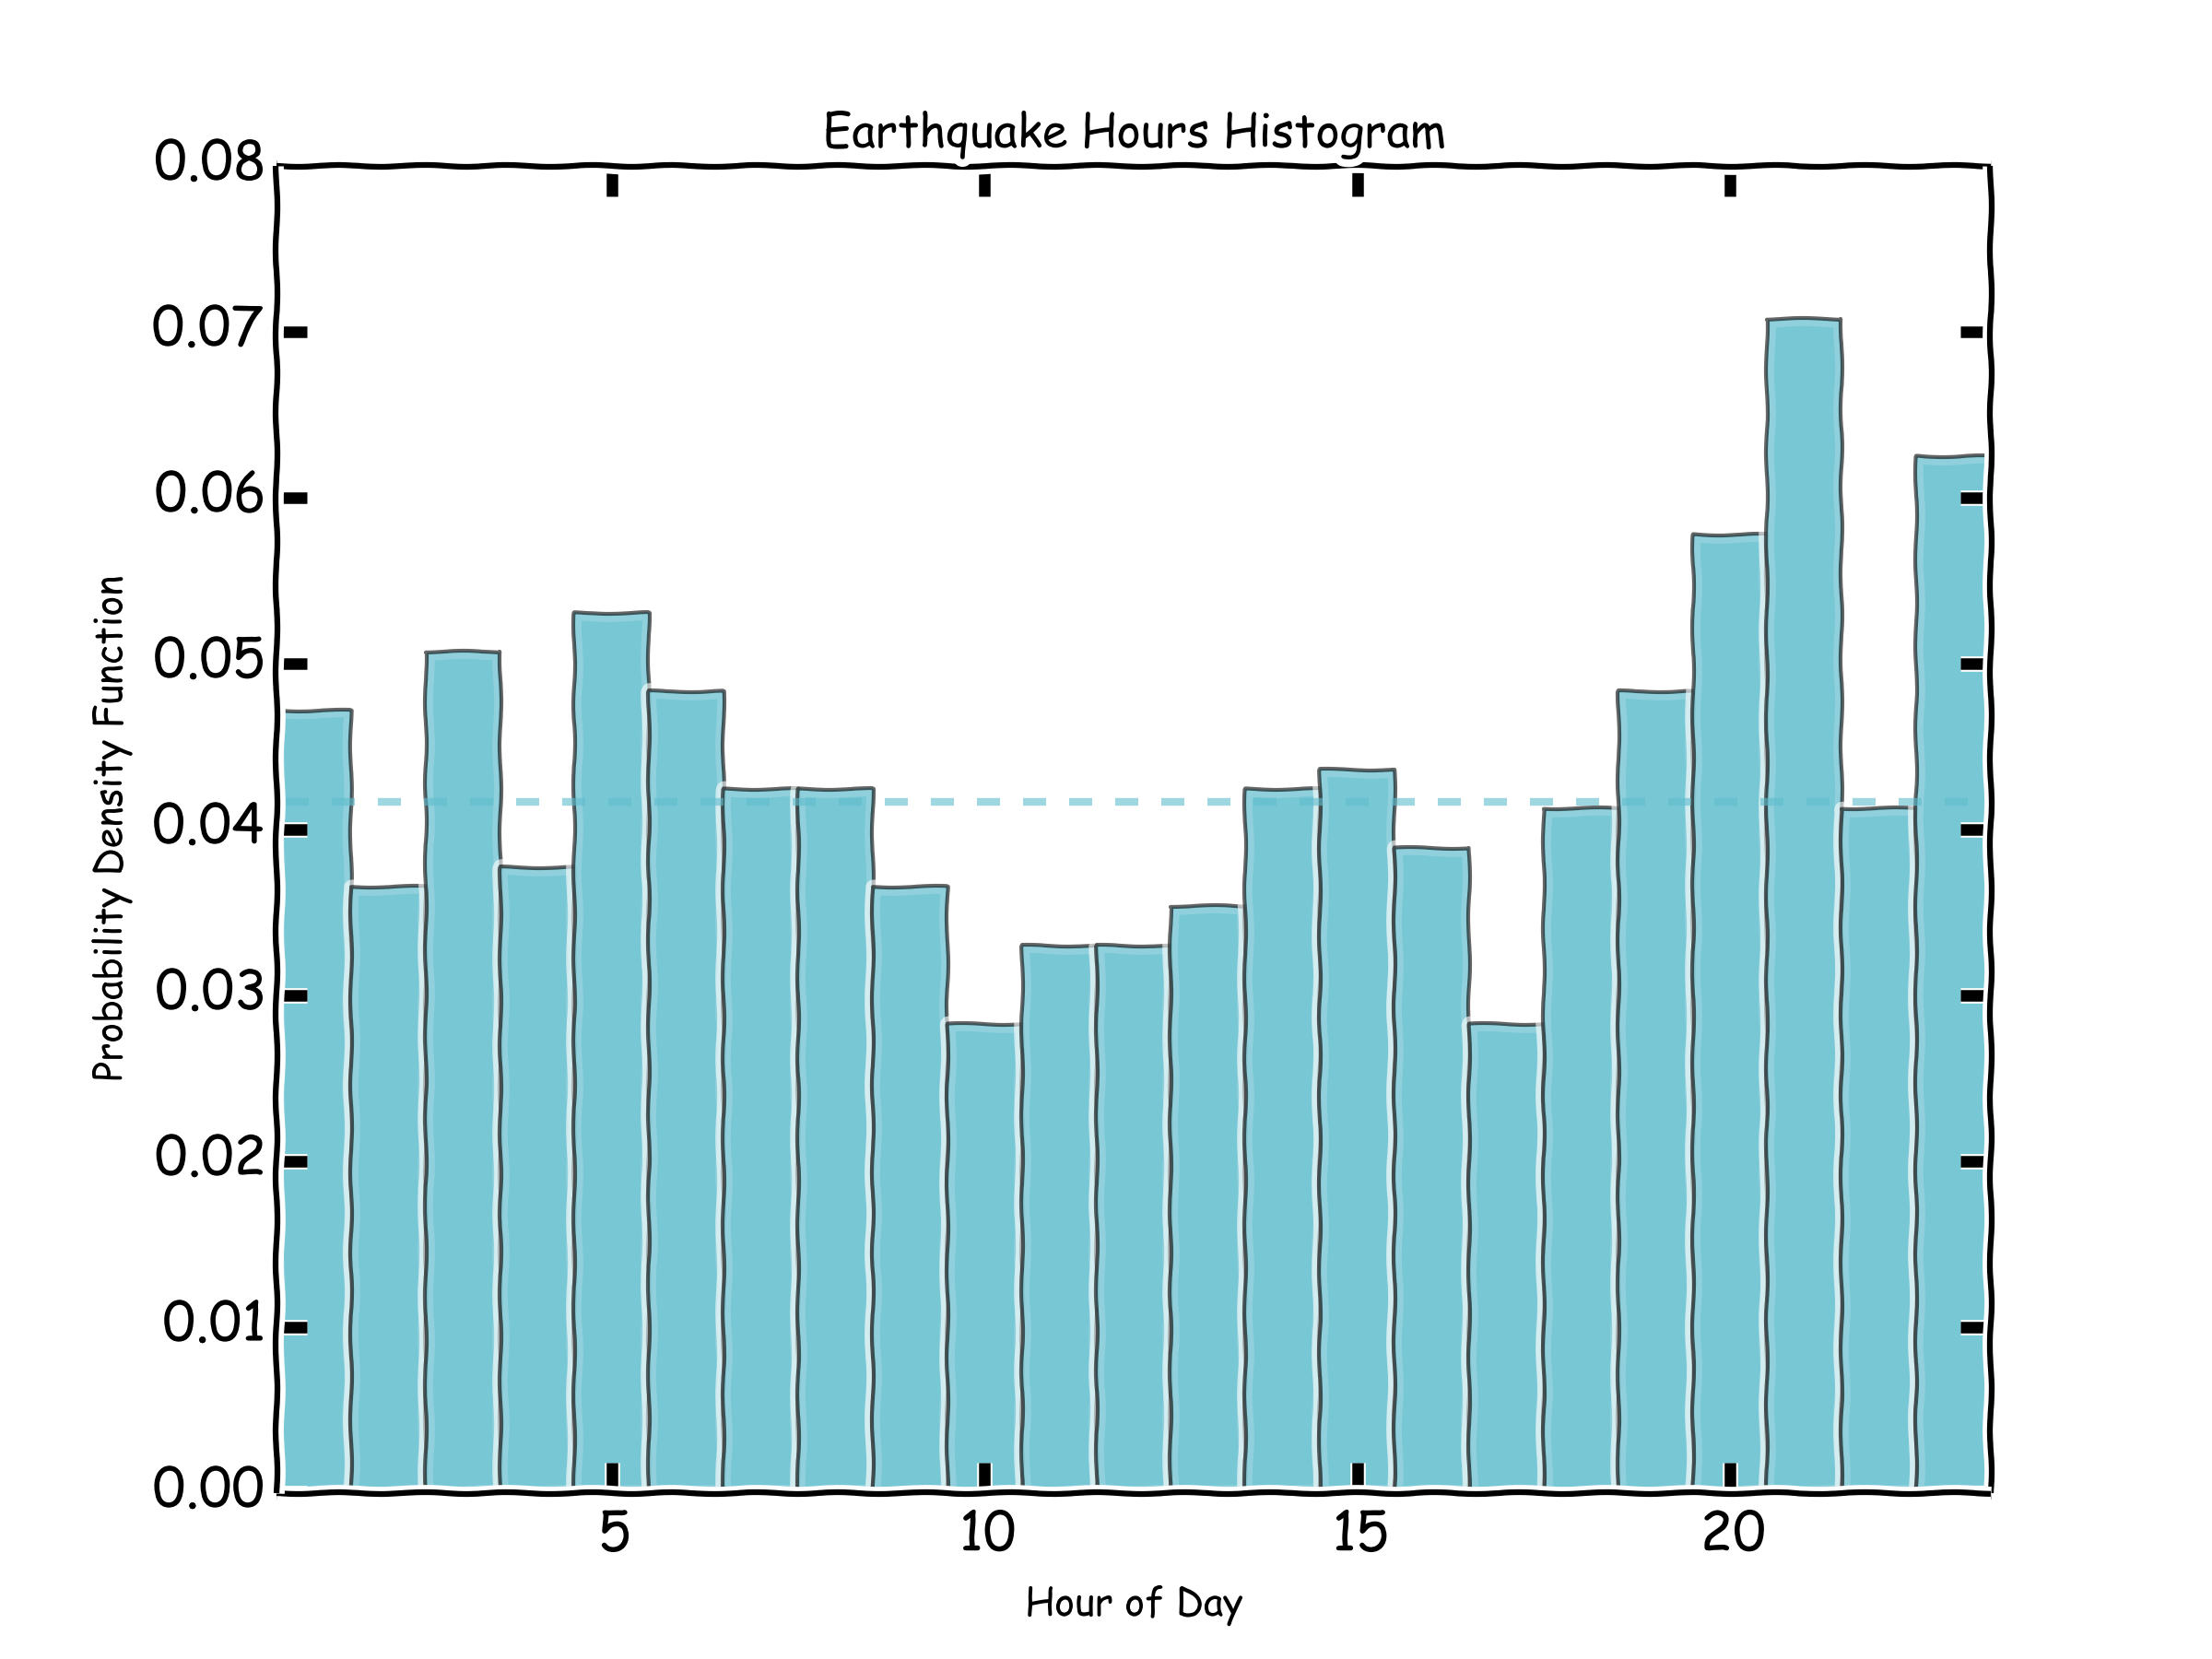
\includegraphics[width=1.00\textwidth]{hmtk_bsb2013_hour}
			\subcaption{Distribuição do horário de ocorrência dos tremores, \gls{bsb2013}}
			\label{fig:br_hour_hist}
    \end{subfigure}%
        %~ %add desired spacing between images, e. g. ~, \quad, \qquad, \hfill etc.
          %(or a blank line to force the subfigure onto a new line)

	\begin{subfigure}[b]{0.45\textwidth}
		  	\centering
			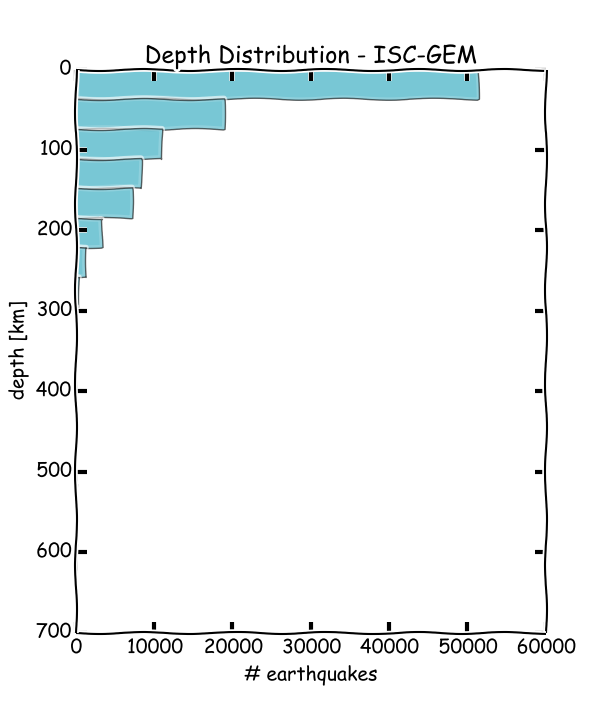
\includegraphics[width=1.00\textwidth]{dep_sa_hist}
			\subcaption{Distribuição da profundidade dos tremores, \gls{iscgem}}
			\label{fig:sa_dep_hist}
	\end{subfigure}%
	\quad %~ %add desired spacing between images, e. g. ~, \quad, \qquad, \hfill etc.
	\begin{subfigure}[b]{0.4\textwidth}
		  	\centering
			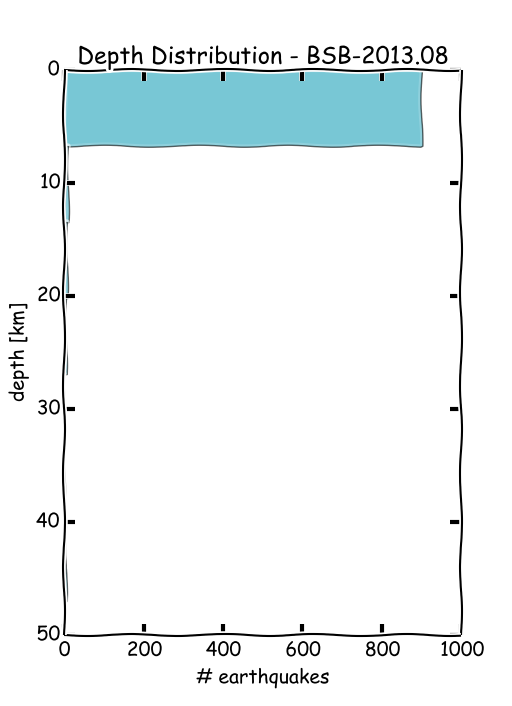
\includegraphics[width=1.00\textwidth]{dep_br_hist}
			\subcaption{Distribuição da profundidade dos tremores, \gls{bsb2013}}
			\label{fig:br_dep_hist}
        \end{subfigure}%
        %~ %add desired spacing between images, e. g. ~, \quad, \qquad, \hfill etc.

  \caption{Checagem de qualidade.}
  \label{fig:qc_histograms} 
\end{figure}

Nas figuras \ref{fig:sa_week_hist} e \ref{fig:br_week_hist} não se observam grandes vieses em 
relação aos dias da semana, nem nos horários de ocorrência durante o dia 
(figuras \ref{fig:sa_week_hist} e \ref{fig:br_week_hist}) nos dois catálogos.

No que diz respeito à distribuição de profundidade, o catálogo do ISC tem as
profundidades mais distribuidas, mesmo com grande maioria sendo eventos rasos 
também se observa um número razoável de sismos a mais de 600km de profundidade.
O BSB por sua vez é composto praticamente todo de sismos rasos, com menos de 10km
de profundidade, ou na prática, com profundidade desconhecida.



%% ------------------------------------------------------------------------- %%
\subsection{Conversão de Magnitudes}
\index{magnitudes!conversão}
\label{sec:mag_conv}

Para que a magnitude dos tremores possam ser analizadas em termos do momento sísmico e do 
tamanho da ruptura que geram é preciso que os sismos do catálogo apresentem pelo menos um valor
\gls{sym:MW} para a magnitude.

No catálogo do ISC-GEM isso é assunto resolvido pois as magnitudes \gls{sym:MW} já foram computadas \citep{storchak_2013}, mas no
caso do \gls{bsb} a maior parte das magnitudes são regionais $m_R$ que se assemelham às magnitudes $m_b$ 
ou magnitudes estimadas a partir de dados macrossísmicos. Nos dois casos é preciso avaliar funções que relacionem os
vários valores de magnitude e \gls{sym:MW}.

Para o catálogo \gls{bsb} as relações conhecidas\footnotetext{por Assumpção,M. e Drouet, S. (não-publicado)} para serem
usadas são as de equivalência entre $m_R$ e $m_b$:
\begin{equation}
	\ensuremath{
		m_R \equiv m_b,
	}
\label{eq:mrmb}
\end{equation}
as de conversão de $m_b$ em $\gls{sym:MW}$
\begin{equation}
	\ensuremath{
		M_W(m_b) = 1.12 m_b + 0.76,
	}
\label{eq:mwmb}
\end{equation}
as de conversão entre $A_f$ e $M_W$
\begin{equation}
	\ensuremath{
		M_W(A_f) = 0.6 + 0.8\log A_f,
	}
\label{eq:mwaf}
\end{equation}
onde \gls{sym:Af} é \glsdesc{sym:Af}; e por fim as estimativas de $m_b$ a partir da \glsdesc{sym:I0} (\gls{sym:I0})
já calculadas quando presentes no catálogo.

NOTA: Essa etapa de pré-processamento, por simplicidade, não foi feita no escopo desse trabalho mas é aqui apresentada 
como referência para trabalhos futuros.


%% ------------------------------------------------------------------------- %%
\subsection{Remoção de agrupamentos}
\index{remoção de agrupamentos}\index{declustering}
\label{sec:declustering}

A maior parte dos modelos de sismicidade estudados assumem que a ocorrência de
tremores segue um processo de Poisson.

Mas sabe-se que os predecessores e sucessores de tremores principais não são independentes.
O aumento do número de sismos pouco antes e pouco depois de um grande tremor contamina
o catálogo com mais sismos do que seriam realmente esperados se os tremores fossem realmente independentes.
Por exemplo, logo após um sismo de magnitude 8, geralmente ocorrem durante um curto 
espaço de tempo mais alguns sismos de magnitude próximo a 7 e cerca de dezenas de sismos 
de magnitude menores que 5, que não ocorreriam com essa mesma frequência na ausência do sismo
principal, de magnitude 8.

Existem outros modelos que usam exatamente essa variação das taxas de sismicidade com o tempo
para fazerem projeções de curto-prazo, mas que não estão no escopo desse trabalho.

Os métodos mais difundidos para a remoção desses agrupamentos não-Poissonianos são métodos que consistem em definir
janelas de tempo e espaço em função da magnitude \citep{gardner_1974}, dentro das quais, os sismos são considerados como pertencentes ao mesmo
agrupamento. 

A seguir estão três formulações implementadas no HMTK para a remoção de agrupamentos.
A primeira de \citet{gardner_1974} é 
\begin{equation}\begin{split} 
\mbox{d(m)} = &10^{0.1238 m + 0.983}\\
\mbox{t(m)} = & 
\begin{cases} 10^{0.032 m + 2.7389} & \text{se $m \geq 6.5$} \\ 
              10^{0.5409 m - 0.547} & \mbox{caso contrário}  \end{cases}\end{split}
\end{equation}

Uma formulação alternativa foi proposta por Gr\"unthal \citep{marsan_david_2012} :

\begin{equation}\begin{split} 
\mbox{d(m)} = & e^{1.77 + \left( {0.037 + 1.02 m} \right)^2} \\ 
   \mbox{t(m)} = & \begin{cases}   |e^{-3.95+ \left( {0.62 + 17.32 m}
    \right)^2}|    & \text{se $m \geq 6.5$ } \\ 10^{2.8 + 0.024 m} & 
    \text{caso contrário}  \end{cases}\end{split}
\end{equation}

E outra sugerida por \citet{uhrhammer_1986}
%
\begin{equation}
\mbox{d(m)} = e^{-1.024 + 0.804 m} \quad \mbox{t(m)} = 
    e^{-2.87 + 1.235 m}
\end{equation}

Enquanto os métodos acima definem explicitamente a janela de tempo, Musson \citet{musson_1999}, propôs que as janelas de tempo
fossem janelas móveis em vez de fixas. Sua teoria é consistente com a de \citet{gardner_1974}.

A figura \ref{fig:eq_decluster_cum} apresenta os resultados de distintos métodos e janelas aplicados aos 
catálogos.

\begin{figure}[H]
	\centering
	\begin{subfigure}[b]{0.48\textwidth}
		  	\centering
			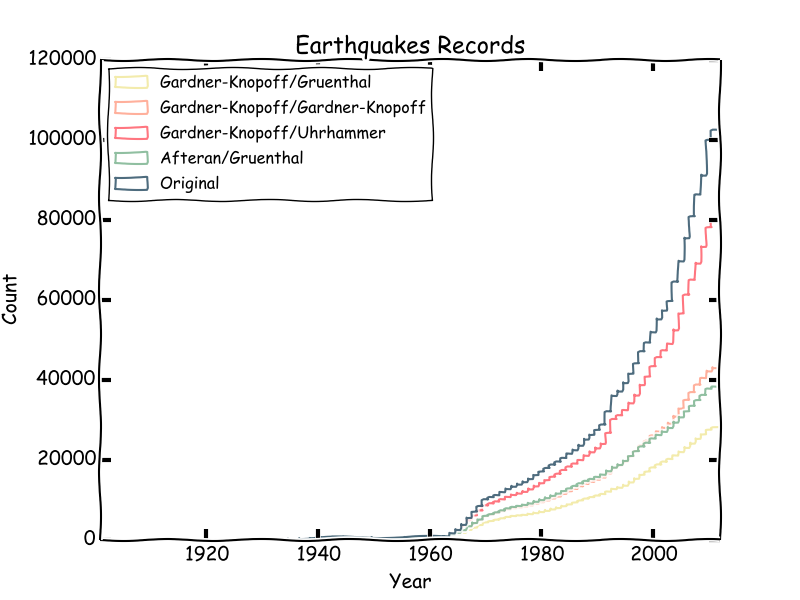
\includegraphics[width=1.00\textwidth]{decluster_sa}
			\subcaption{Número cumulativo de tremores registrados por ano para o \gls{iscgem}
			original e para diferentes métodos/janelas de remoção de agrupamentos.}
			\label{fig:sa_eq_record}
	\end{subfigure}%
	\quad %~ %add desired spacing between images, e. g. ~, \quad, \qquad, \hfill etc.
	\begin{subfigure}[b]{0.48\textwidth}
		  	\centering
			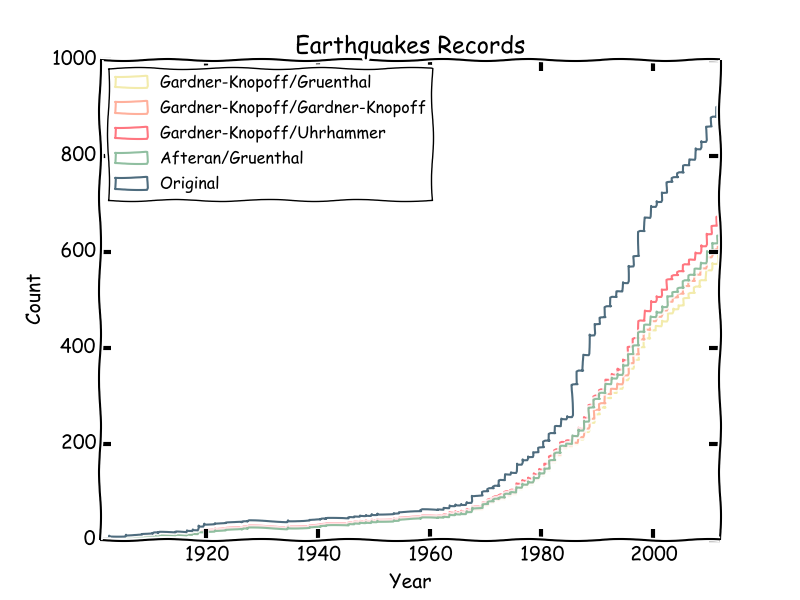
\includegraphics[width=1.00\textwidth]{decluster_br}
			\subcaption{Número cumulativo de tremores registrados por ano para o \gls{bsb2013}
			original e para diferentes métodos/janelas de remoção de agrupamentos.}
			\label{fig:br_eq_record}
    \end{subfigure}%
	\caption{Número cumulativo de tremores registrados por ano após 1900}
	\label{fig:eq_decluster_cum}
\end{figure}

No caso do \gsl{bsb2013} os resultados são relativamente equivalentes quando comparados aos resultados no caso do 
\glsdesc{iscgem}, onde é possível notar claramente as diferenças nos resultados de cada método de remoção de
agrupamento. Isso demonstra que uma discussão mais aprofundada sobre os métodos de 
remoção de agrupamentos é necessária mas está além dos propósitos desse texto.

A figura \ref{fig:eq_decluster} ilustra os agrupamentos de sismos não-Poissonianos encontrados 
pelo método de AFTERAN \citep{musson_2000} e janelas de Gr\"uenthal quando aplicados
aos catálogos \gls{iscgem} e \gls{bsb2013}. As sequencia de cores indica o número de cada agrupamento, e sua
distribuição espacial não apresenta qualquer padrão. 

\begin{figure}[H]
	\centering
	\begin{subfigure}[t]{0.46\textwidth}
		  	\centering
			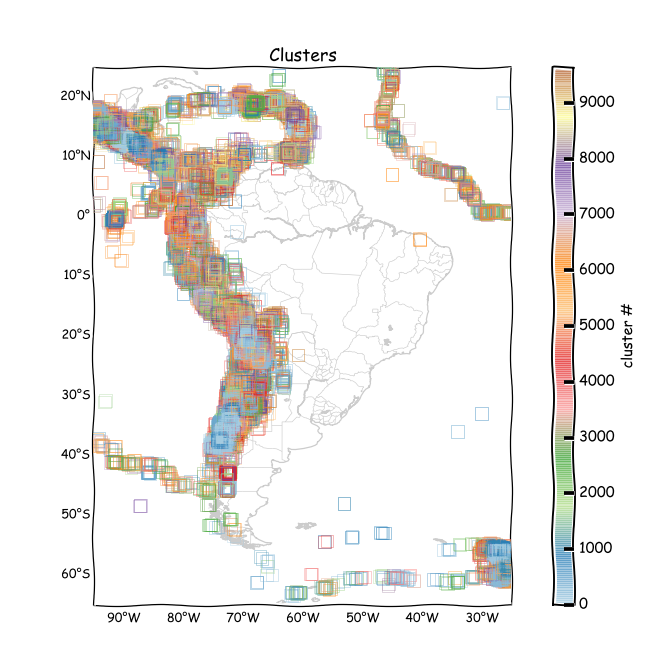
\includegraphics[width=1.00\textwidth]{hmtk_sa3_pp_decluster}
			\subcaption{Número de tremores registrados por ano, \gls{iscgem}}
			\label{fig:sa_decluster}
	\end{subfigure}%
	\quad %~ %add desired spacing between images, e. g. ~, \quad, \qquad, \hfill etc.
	\begin{subfigure}[t]{0.50\textwidth}
		  	\centering
			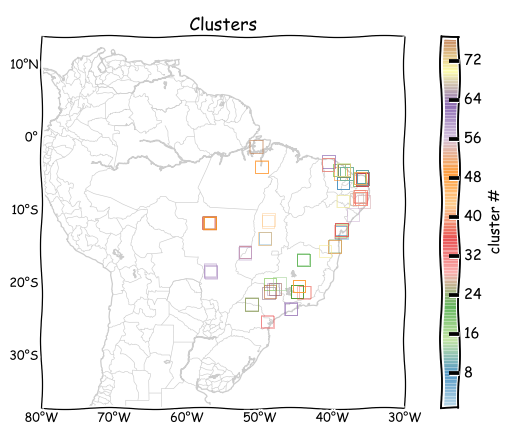
\includegraphics[width=1.00\textwidth]{hmtk_bsb2013_pp_decluster}
			\subcaption{Número de tremores registrados por ano, \gls{bsb2013}}
			\label{fig:br_decluster}
    \end{subfigure}%
	\caption{Número de tremores registrados por ano após 1900}
	\label{fig:eq_decluster}
\end{figure}

Os catálogos com os agrupamentos removidos passam a ser os catálogos utilizados nas etapas posteriores.

%% ------------------------------------------------------------------------- %%
\subsection{Análise da Magnitude de Completude}
\index{Magnitude de Completude}
\label{sec:completeness}

Uma evidência da necessidade de se avaliar a magnitude de completude \gls{sym:Mc}
pode ser percebida ao contar a quantidade de sismos registrados ao longo do tempo
para cada intervalo de magnitude. A figura \ref{fig:qc_time_mag_count} apresenta
esses gráficos para os catálogos considerados.

\begin{figure}[H]
	  \centering
	  \begin{subfigure}[b]{0.7\textwidth}
		  	\centering
			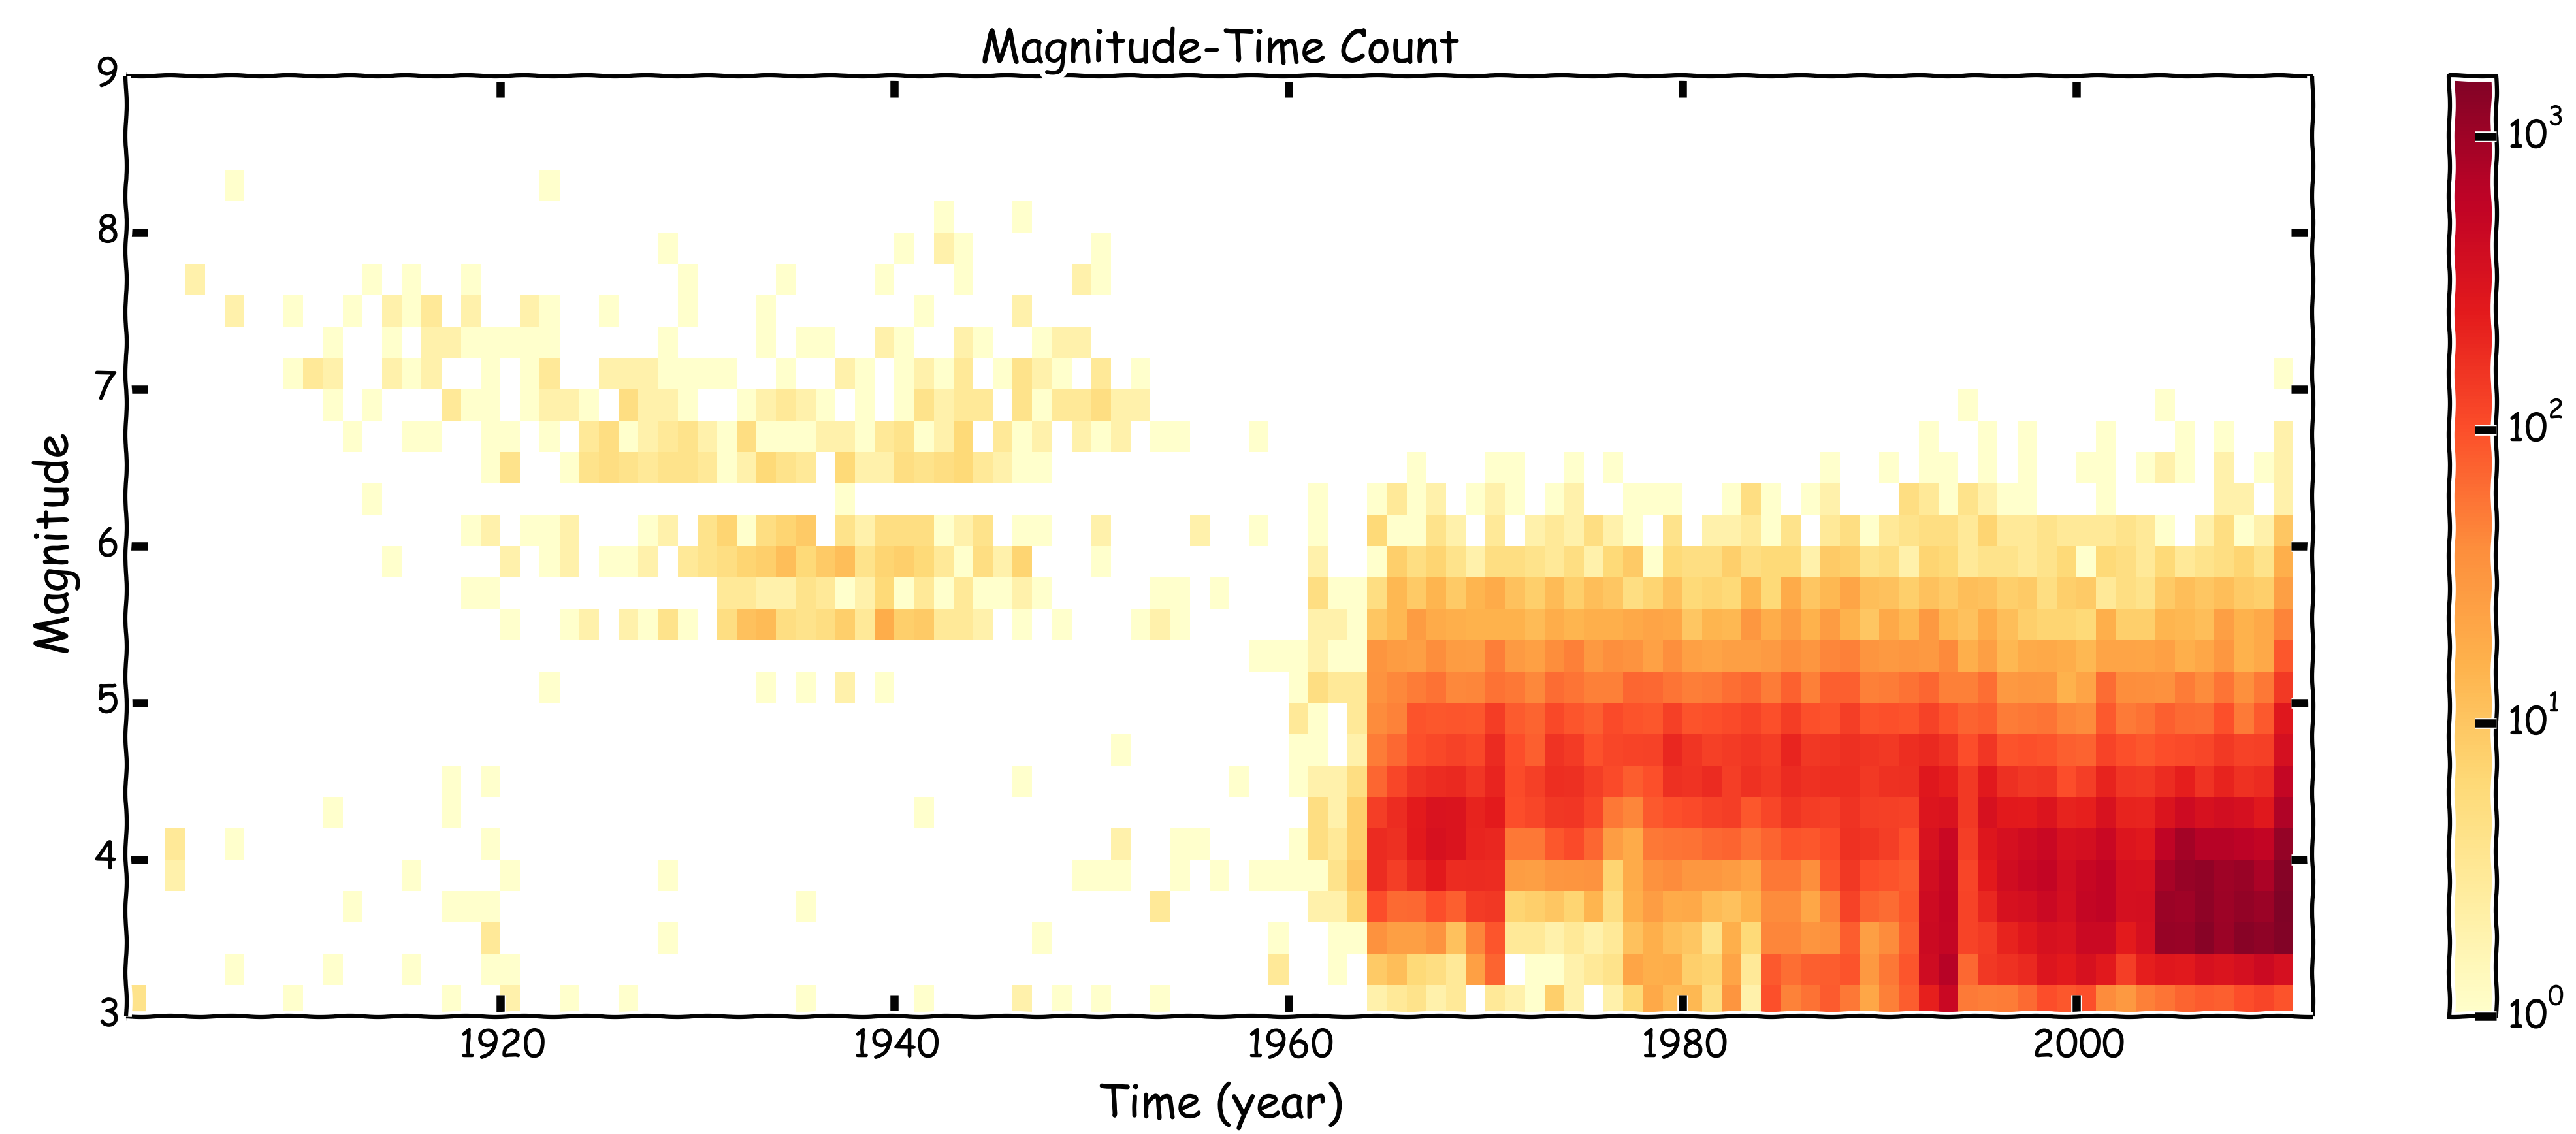
\includegraphics[width=1.00\textwidth]{time_mag_count_sa}
			\caption{Catálogo \gls{iscgem} 1900-2012}
			\label{fig:tmf_sa}
        \end{subfigure}%
        %~ %add desired spacing between images, e. g. ~, \quad, \qquad, \hfill etc.
          %(or a blank line to force the subfigure onto a new line)

	  \begin{subfigure}[b]{0.7\textwidth}
		  	\centering
  			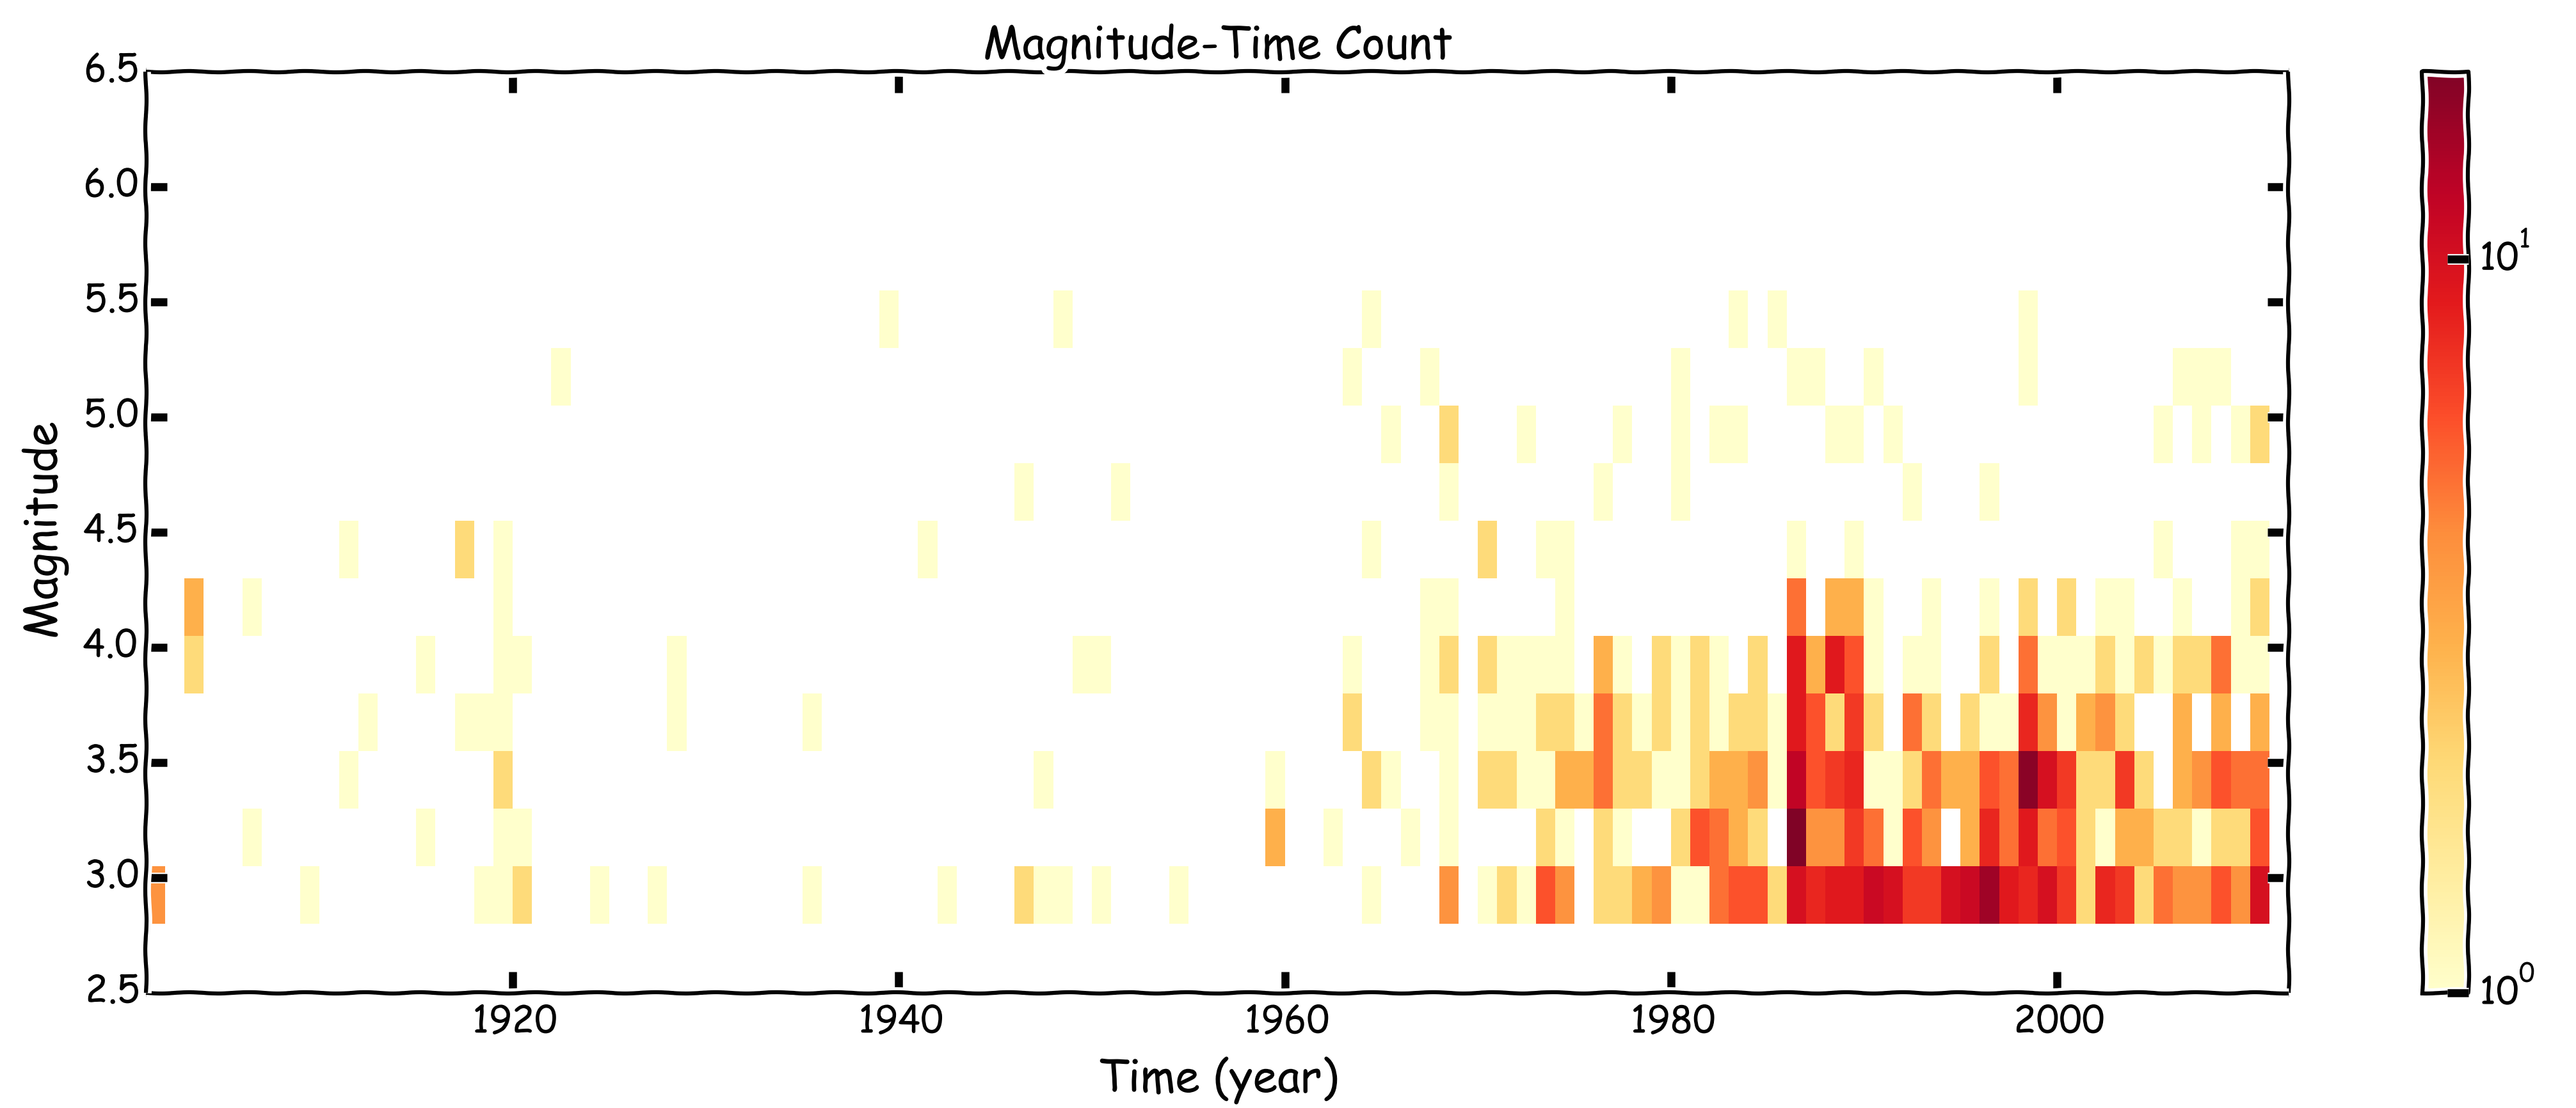
\includegraphics[width=1.00\textwidth]{time_mag_count_br}
			\caption{Catálogo \gls{bsb2013} 1900-2012}
			\label{fig:tmf_br}
       \end{subfigure}%

	   \begin{subfigure}[b]{0.7\textwidth}
		  	\centering
  			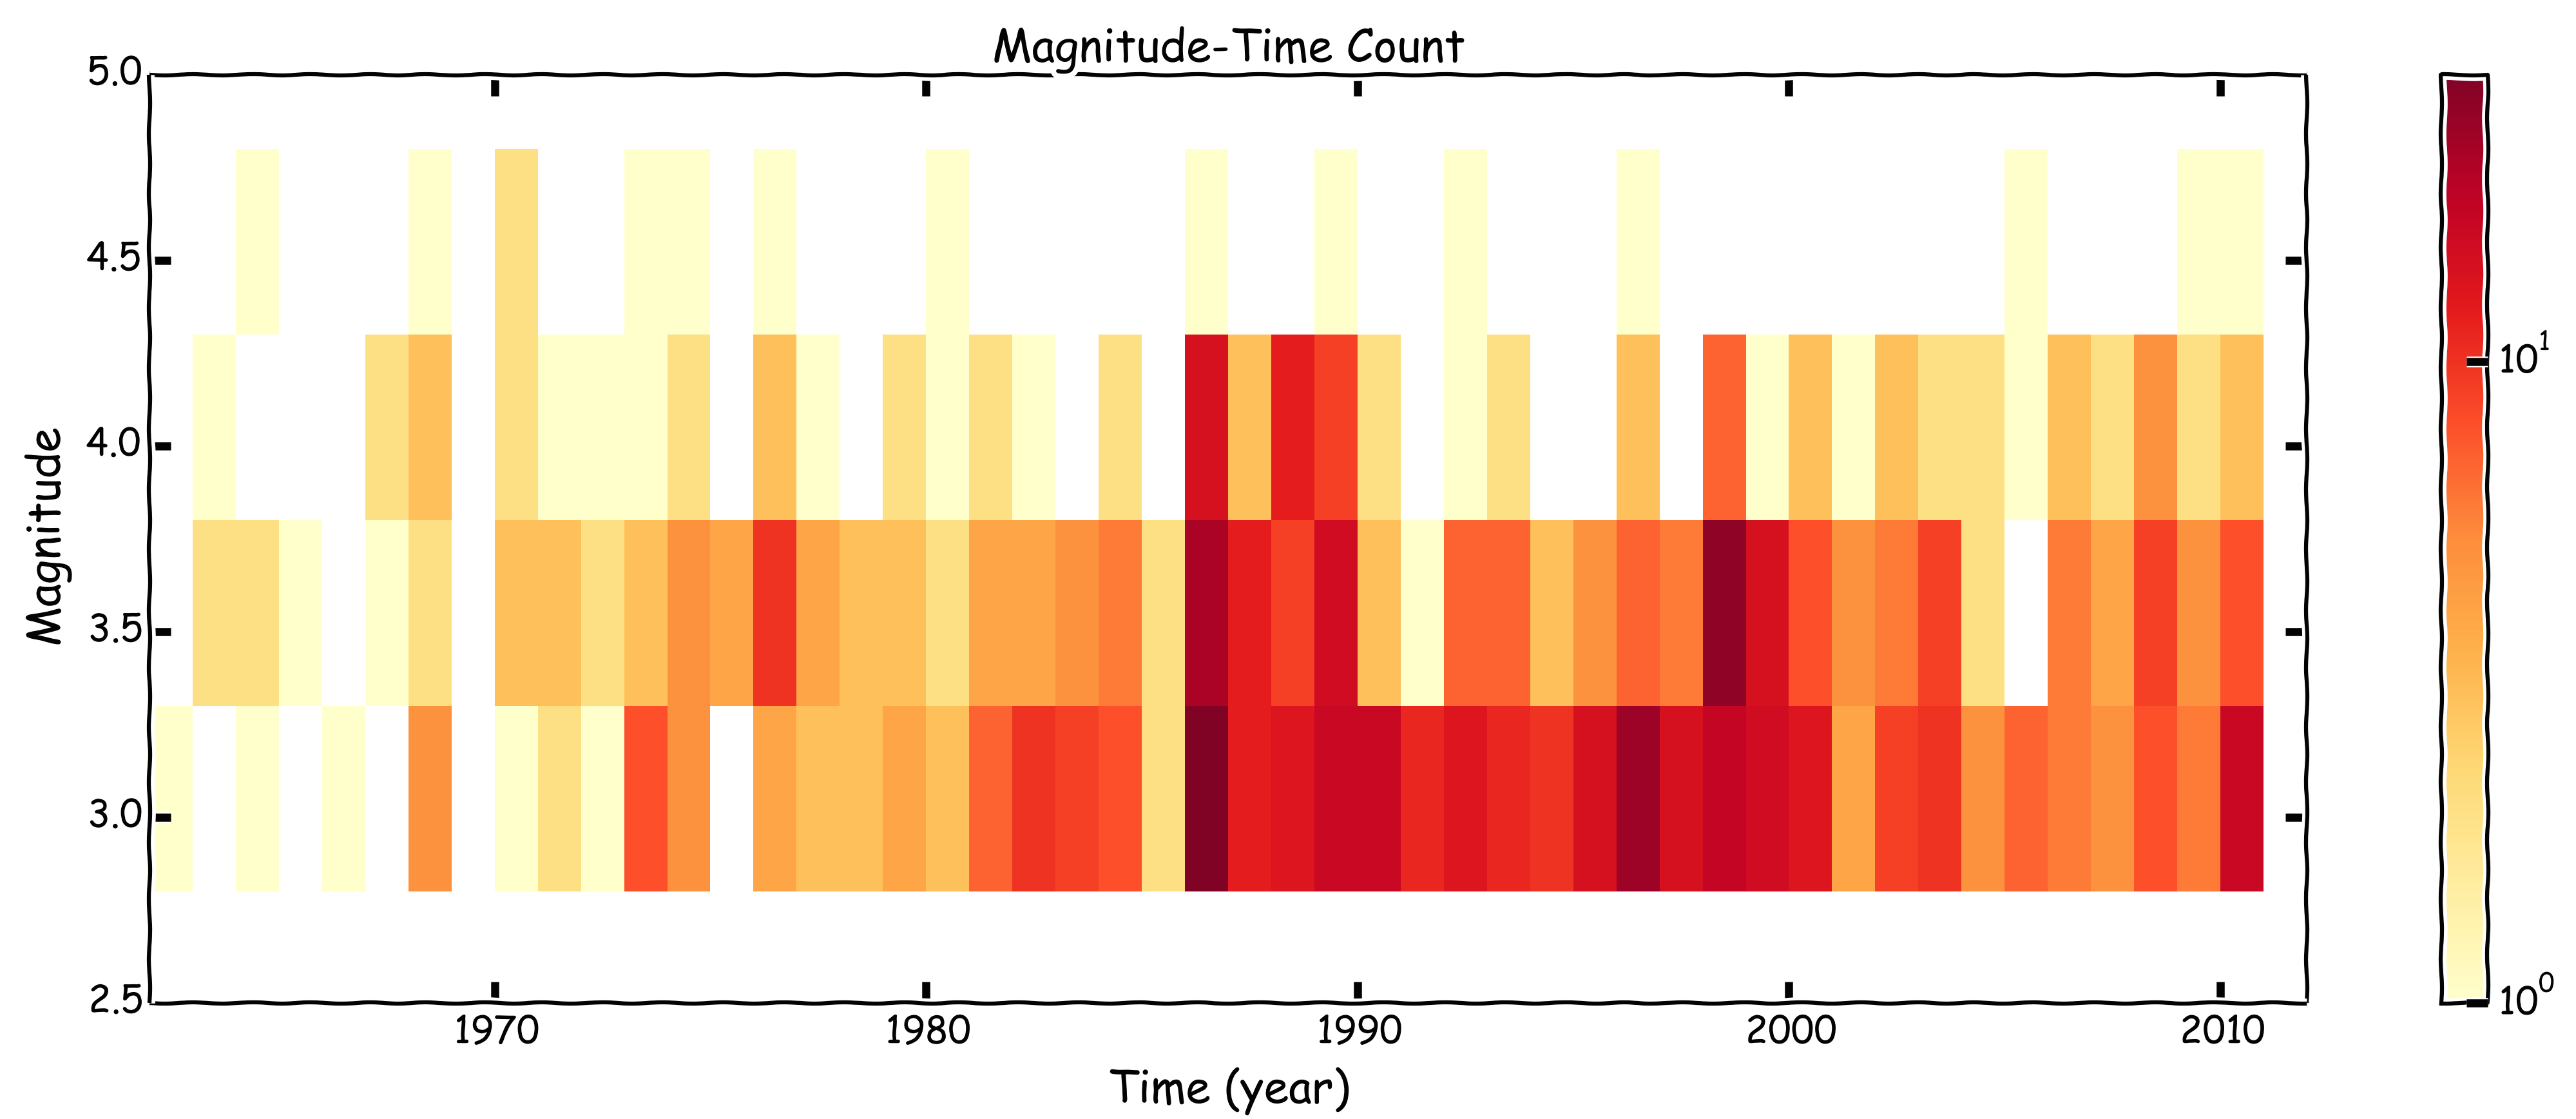
\includegraphics[width=1.00\textwidth]{time_mag_count_br_1960}
			\caption{Catálogo \gls{bsb2013} a partir de 1960-2012}
			\label{fig:tmf_br_1960}
       \end{subfigure}%

  \caption{Contagem de sismos em tempo e em magnitude.}
  \label{fig:qc_time_mag_count} 
\end{figure}

Na figura \ref{fig:qc_time_mag_count} é possível perceber, nos dois catálogos,
que a quantidade de sismos no mesmo intervalo de magnitude varia bastante ao longo do tempo.
Isso se deve à uma série de fatores, mas principalmente à capacidade de registro
da rede sismográfica, implantação de redes globais e 
à modernização e aumento de sensibilidade de equipamentos.

A magnitude de completude é importante \citep{woessner_2005} por sua influência direta no cálculo dos parâmetros $a$ e
$b$ de Gutemberg-Richter.
Ela pode variar ao longo do tempo e do espaço (variação da densidade de estações sismográficas).


\begin{p}
\textbf{Stepp Test}
\end{p}

O método de \citet{stepp_1971} permite obter a variação temporal da magnitude
de completude \gls{sym:Mc} diretamente à partir do catálogo com um teste simples.

Esse procedimento analítico foi um dos primeiros a serem propostos para esse fim.
Sejam $\lambda_1, \lambda_2, \cdots, \lambda_n$ o número de sismos por unidade de tempo.
Assumindo que os tremores de certa faixa de magnitude têm distribuição de Poisson, a estimativa da taxa de
média de sismicidade $\lambda$ por unidade de tempo é expressa por

\begin{equation}
	\ensuremath{
		\lambda =  \frac{1}{n}\sum_{i=1}^{n} \lambda_i.
	}
\label{eq:mwaf}
\end{equation}
Sua variância $\sigma_{\lambda}^2 =  \lambda/n$, com $n$ o número de intervalos.

Com intervalos de 1 ano, $n$ intervalos é o período $T$ de observação com desvio padrão
\begin{equation}
	\ensuremath{
		 \sigma_{\lambda} = \frac{\sqrt{\lambda}}{\sqrt{T}}.
	}
\label{eq:mwaf}
\end{equation}

A taxa de sismicidade sendo estacionária, seu desvio padrão deve se comportar como $1/\sqrt{T}$ em 
tempos de observação crescentes $T$.

Os diagramas abaixo tomam intervalos de observação crescentes com passo de 2.5 anos,
em intervalos de 0.5 de magnitude.
\begin{figure}[H]
	\centering
	\begin{subfigure}[b]{0.47\textwidth}
		  	\centering
			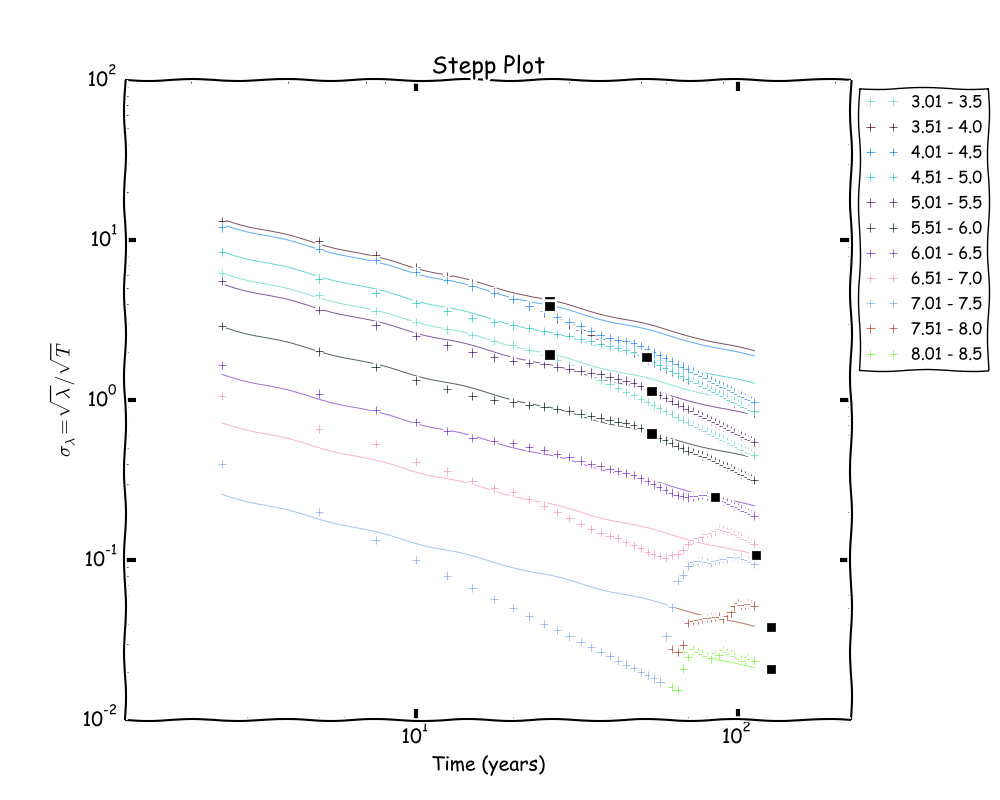
\includegraphics[width=1.00\textwidth]{stepp_sa}
			\subcaption{Diagrama de Stepp para o \gls{iscgem} (\emph{declustered})}
			\label{fig:sa_stepp}
	\end{subfigure}%
	\quad %~ %add desired spacing between images, e. g. ~, \quad, \qquad, \hfill etc.
	\begin{subfigure}[b]{0.47\textwidth}
		  	\centering
			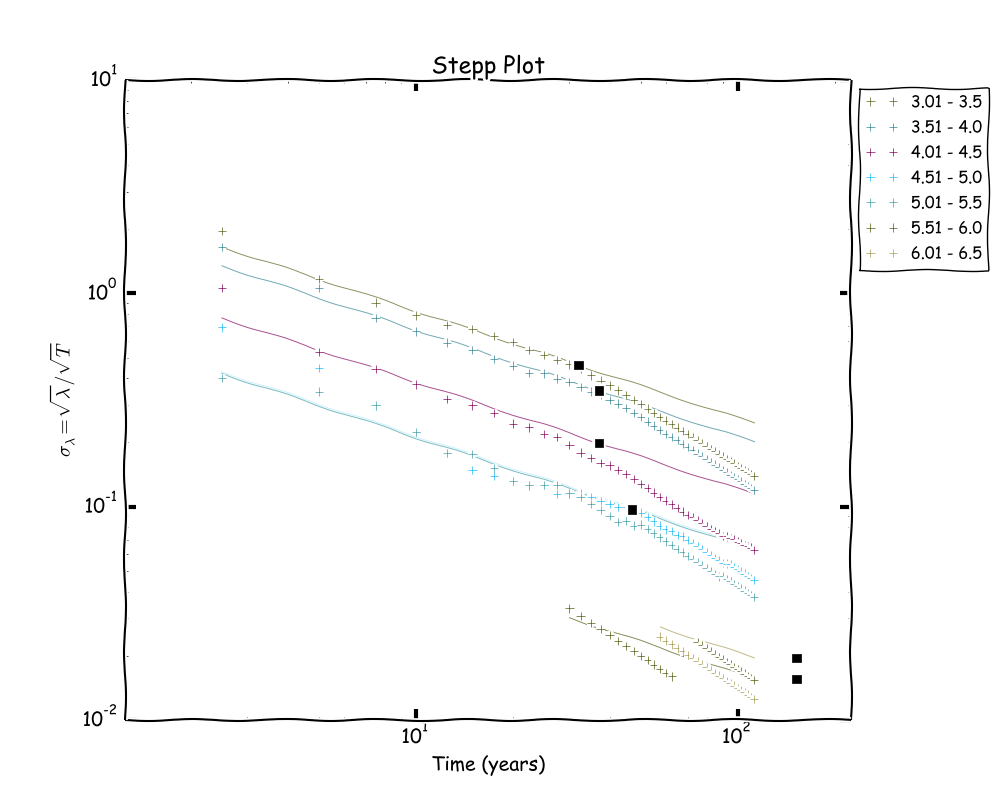
\includegraphics[width=1.00\textwidth]{stepp_br}
			\subcaption{Diagrama de Stepp para o \gls{bsb2013} (\emph{declustered})}
			\label{fig:br_stepp}
    \end{subfigure}%
	\caption{Diagrama de Stepp para análise da magnitude de completude \gls{sym:Mc}}
	\label{fig:eq_stepp}
\end{figure}

Com esses parâmetros, as magnitudes de completude \gls{sym:Mc}, determinadas pelo método
de Stepp, estão listadas nas tabelas \ref{tab:mc_sa} e \ref{tab:mc_br}.

	\begin{table}[h]
	  	\centering
		\begin{tabular}{l|*{11}{c}}
		$M_c$ & 3.0  & 3.5  & 4.0  & 4.5  & 5.0  & 5.5  & 6.0  & 6.5  & 7.0  & 7.5  & 8 \\  \hline
		Ano   & 1986 & 1986 & 1986 & 1960 & 1958 & 1958 & 1927 & 1898 & 1885 & 1885 & 1885   \\
		\end{tabular}
		\caption{Magnitude de completude, \gls{iscgem}}
		\label{tab:mc_sa}
	\end{table}

	\begin{table}[h]
	  	\centering
		\begin{tabular}{l|*{7}{c}}
		$M_c$ & 3.0  & 3.5  & 4.0  & 4.5  & 5.0  & 5.5  & 6.0  \\  \hline
		Ano   & 1980 & 1975 & 1975 & 1965 & 1965 & 1860 & 1860 \\
		\end{tabular}
		\caption{Magnitude de completude, Cat.BSB2013}
		\label{tab:mc_br}
	\end{table}

Os parâmetros a serem utilizados podem ser controversos, inclusive a opção de forçar com que 
os anos de completude de magnitudes maiores sejam ao menos iguais aos de magnitude menores, 
mas novamente, a discussão sobre os melhores parâmetros para o método de Stepp, sua validade, ou 
mesmo outros métodos estão além da proposta desse texto.

Os valores de \gls{sym:Mc} das tabelas \ref{tab:mc_sa} e \ref{tab:mc_br} são os valores utilizados
no cálculo da recorrência no resto do trabalho.


%% ------------------------------------------------------------------------- %%
\section{Frankel, 1995}
\index{Frankel, 1995!processamento}
\label{sec:proc_frankel}

Tanto no método de Frankel como nos demais métodos avaliados,
a malha para a estimativa de taxa de sismicidade para o Brasil 
foi de $1^o \times 1^o$, o \emph{valor-b} foi fixado em 1.

Para o processamento pelo método de Frankel, utilizou-se o catálogo com os agrupamentos removidos,
e a tabela de magnitude de completude menciona. A distância de correlação utilizada foi 
de 150km. A zona de influência foi limitada em 3 vezes a distância de correlação.

%% ------------------------------------------------------------------------- %%
\section{Woo, 1996}
\index{Woo, 1996!processamento}
\label{sec:proc_woo}

O processamento pelo método de Woo também foi feito com a remoção dos agrupamentos no catálogo.

A largura de banda dependente da magnitude é ajustada pelo próprio método.
O ajuste da função de largura de banda é apresentado na figura~\ref{fig:woo_b} para o \gls{bsb2013}:

\begin{figure}[H]
  \centering
  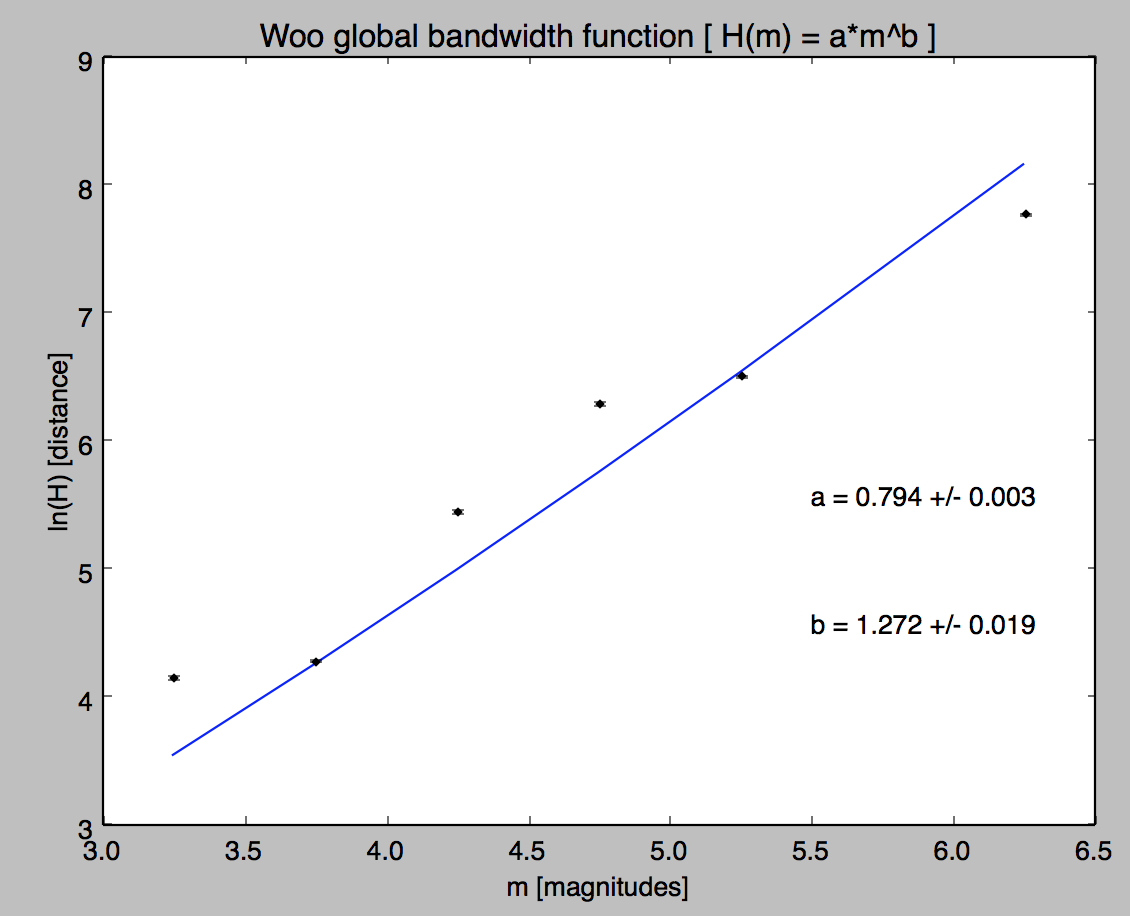
\includegraphics[width=.80\textwidth]{woo_bandwidth} 
  \caption{Ajuste da largura de banda para o método de Woo1996}
  \label{fig:woo_b} 
\end{figure}

Apenas como comparação estão apresentados também os ajustes citados por \citet{beauval_2003} para a Espanha e Noruega.
Como é possível observar o ajuste brasileiro apresenta distâncias médias sistematicamente maiores, provavelmente
devido à escala continental do Brasil.

A função de núcleo utilizada foi a proposta pela equação \eqref{eq:k_kj}.

%% ------------------------------------------------------------------------- %%
\section{Helmstetter, 2012}
\index{Helmstetter!processamento}
\label{sec:proc_helmstetter}

Utilizou-se, para a projeção da taxa de sismicidade, como catálogo de teste
um filtro para o catálogos o período 1950-2007. Os sismos de 2007-2012 juntamente
com os sismos ocorridos antes de 1950 foram colocados no catálogo-alvo.

A escolha por colocar os sismos anteriores à 1950 no catálogo se deve à estabilidade
da crosta no Brasil e da pouca capacidade histórica de observação,
esses poucos sismos trazem informações importantes sobre essas fontes
sismogênicas que não aparecem no catálogo no periodo escolhido para a aprendizagem.

Para a aprendizagem foram utilizados sismos com magnitudes acima de 3.8 buscando projeções para
sismos com magnitudes acima de 4.0.

A figura \ref{fig:h_catalogue} apresenta os catálogos de treino e de teste usados na otimização.

\begin{figure}[H]
  \centering
  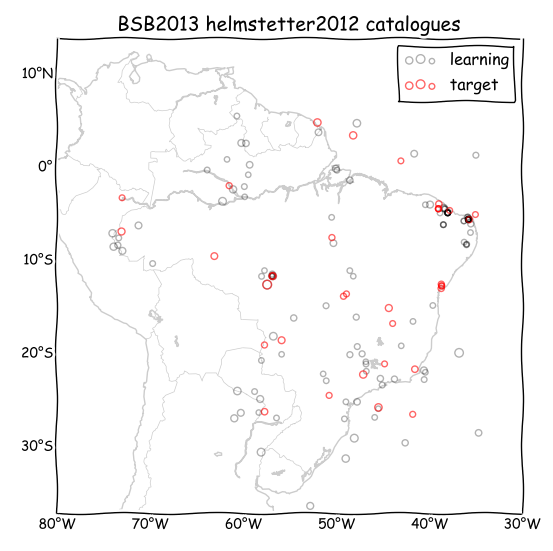
\includegraphics[width=.80\textwidth]{helmstetter_catalogues} 
  \caption{Catálogos de aprendizado e de teste para o método de \citet{helmstetter_2012}}
  \label{fig:h_catalogue} 
\end{figure}

As magnitudes de completude, embora haja espaço no modelo para sua representação espacial e temporal
e, teoricamente, pudessem ser calculadas para o instante e posição de cada sismo para que fossem
considerados com os pesos adequados, não foram consideradas dessa forma. Em vez disso a magnitude
de completude utilizada foi a mínima magnitude no catálogo de teste ($m=3.8$) uniformemente para todo o catálogo.

Os cálculos da largura de banda $h_i$ e $d_i$ de cada sismo é ilustrado no caso de um evento particular na figura
\ref{fig:h_hidi}.

\begin{figure}[H]
  \centering
  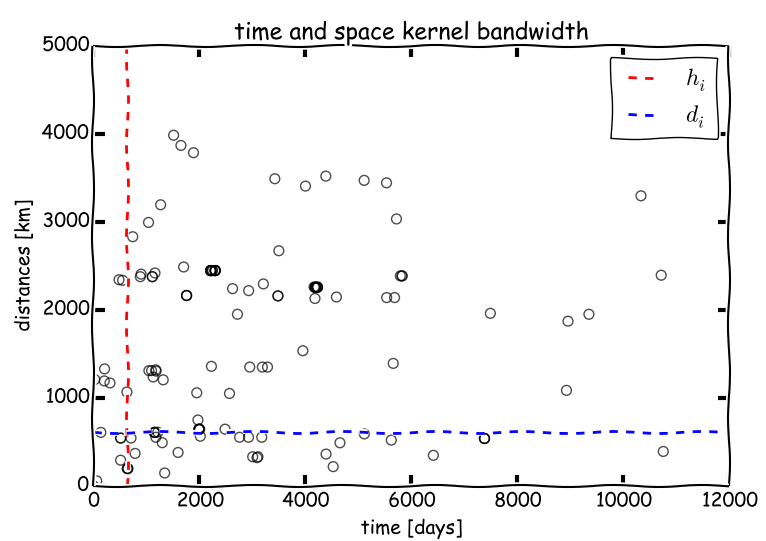
\includegraphics[width=.80\textwidth]{helmstetter_hidi} 
  \caption{Exemplo da largura de banda para um determinado evento para o método de Helmstetter, com $k_{cnn} = 5$ e
  $a_{cnn} = 100$}
  \label{fig:h_hidi} 
\end{figure}

Nota-se que as larguras de banda são escolhidas de forma a deixar $k_{cnn}$ eventos entre $h_i$ e $d_i$.

A taxa estacionária em cada célula é calculada a partir da mediana da taxa prevista pelo modelo em cada célula,
como na figura \ref{fig:h_stationary}.
\begin{figure}[H]
  \centering
  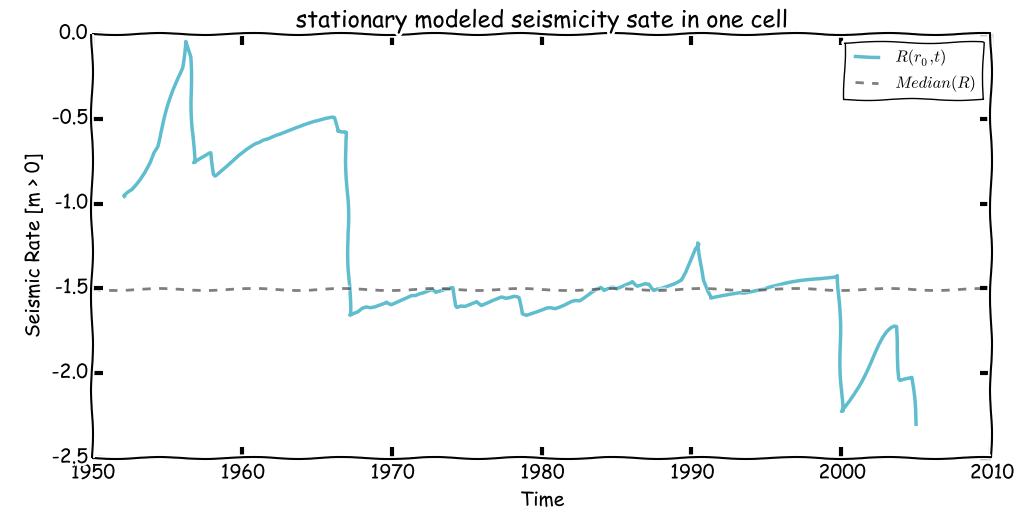
\includegraphics[width=.80\textwidth]{helmstetter_stationary_a} 
  \caption{Taxa de sismicidade estacionaria calculara a partir da mediana da taxa de sismicidade
  modelada pelo método de Helmstetter2012 para uma determinada célula $r_0$}
  \label{fig:h_stationary} 
\end{figure}
A célula em questão fica próxima à região de Mato Grosso e o pico de sismicidade em torno de 1955,
ocorre justamente na época do grande tremor da região.

A função de núcleo utilizada na dimensão do espaço foi a gaussiana \eqref{eq:kernel_gs} multivariada, 
e univariada na dimensão do tempo.

%% ------------------------------------------------------------------------- %%
\section{Pós-Processamento}
\index{pós-processamento}
\label{sec:pos_proc}

Como o objetivo desse trabalho é a caracterização das fontes sísmogênicas,
o cálculo da ameaça pelo método clássico propriamente dito
acaba figurando como pós-processamento.

A figura \ref{fig:classical_psha} apresenta o fluxograma de trabalho para uma análise clássica de \gls{psha} conforme
implementado no Openquake \citep{pagani_2010, weatherill_2012}.

\begin{figure}[H]
	\centering
	\begin{tabular}{l}
	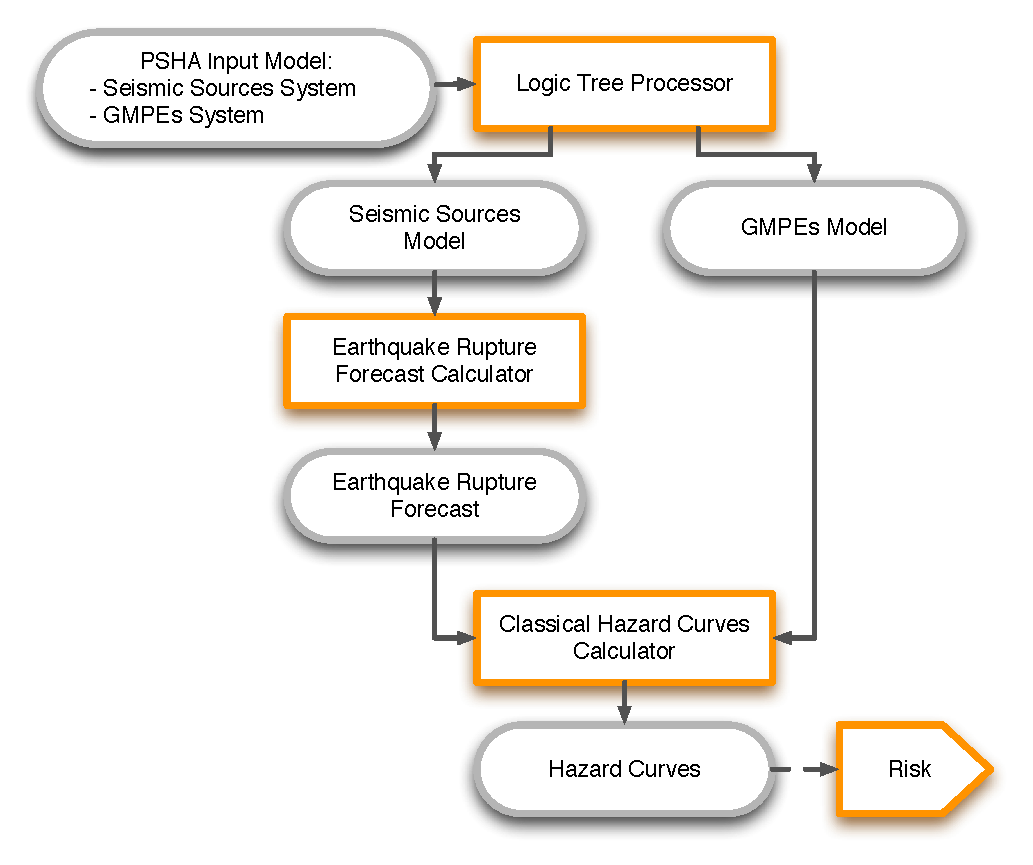
\includegraphics[width=0.80\textwidth]{classical_psha_workflow}
	\end{tabular}
	\caption{Fluxo de trabalho clássico para a \gls{psha} \citep{crowley_2013}.}
\label{fig:classical_psha}
\end{figure}
